\chapter{Radiation Transport and Mobile Depletion in Gnat} 
\label{solver}

This chapter describes the mathematics and implementation of the multiphysics radiation transport and mobile depletion solver generated by this work. Section~\ref{solver:radiation_transport} discusses the mathematics of neutral particle transport, derives a energy-space-angle discretization of the transport equation suitable for implementation in \acrshort{moose}, and provides a discussion surrounding ray effect mitigation measures. Section~\ref{solver:depletion} provides the mobile depletion equations and derives both a \acrshort{cgfem} and \acrshort{fvm} discretization. Finally, Section~\ref{solver:implementation} discusses the approach taken to implement these solvers in the \acrshort{moose} framework and the methodology used to couple these solvers together. This includes the nuclear data interface, the implemented \acrshort{moose} objects, solver-solver interfacing, and several utilities which automate the setup of radiation transport and mobile depletion problems. 

\section{The Radiation Transport Solver}
\label{solver:radiation_transport}

The balance of neutral particles in many nuclear systems can be written with the linear Boltzmann equation. Consider an open convex 3D spatial domain $V$ with boundary $\partial V$, 2D unit sphere $\mathcal{S} = [0, \pi] \times [0, 2\pi]$, 1D energy domain $[0, \infty]$, and 1D temporal domain $[t_{0}, t_{1}]$:
\begin{equation}\label{eq:generic_transport_equation}
    \underbrace{\frac{\partial}{\partial t}\frac{\psi(\vec{r}, \hat{\Omega}, E, t)}{v(E)}}_{\text{Time Derivative Term}}
    = \underbrace{\mathbb{S}(\vec{r}, \hat{\Omega}, E, t)}_{\text{Particle Source Term}} 
    - \underbrace{\hat{\Omega}\cdot\vec{\nabla}\psi(\vec{r}, \hat{\Omega}, E, t) }_{\text{Streaming Term}}  
    - \underbrace{\Sigma_{t}(\vec{r}, E, t)\psi(\vec{r}, \hat{\Omega}, E, t)}_{\text{Collision Term}} \text{,}
\end{equation}
where:

\begin{tabular}{rl}
    $\vec{r} = \{x,y,z\}, \vec{r} \in V$             & is the independent spatial variable [cm];\\
    $\hat{\Omega} = \{\theta, \omega\}, \hat{\Omega}\in \mathcal{S}$ & is the independent directional variable [st (steradians)]. Often \\
    &expanded as a vector of direction cosines: $\hat{\Omega} = \{\mu, \eta, \xi\}$, $\mu = \cos\theta$, \\
    & $\eta = \sqrt{1 - \mu^2}\cos\omega$, $\xi = \sqrt{1 - \mu^2}\sin\omega$;\\
    $E\in [0, \infty]$                               & is the independent energy variable [eV];\\
    $t\in [t_{0}, t_{1}]$                            & is the independent time variable [s];\\
    $v(E)$                                           & is the particle speed [cm s\textsuperscript{-1}];\\
    $\psi(\vec{r}, \hat{\Omega}, E, t)$              & is the angular particle flux [cm\textsuperscript{-2} s\textsuperscript{-1} st\textsuperscript{-1} eV\textsuperscript{-1}];\\
    $\Sigma_{t}(\vec{r}, E, t)$                      & is the total macroscopic cross section [cm\textsuperscript{-1}];\\
    $\mathbb{S}(\vec{r}, \hat{\Omega}, E, t)$        & is a particle source [cm\textsuperscript{-3} s\textsuperscript{-1} st\textsuperscript{-1} eV\textsuperscript{-1}] \cite{computational_methods}.
\end{tabular}
\newline

The term on the left of Eq.~\ref{eq:generic_transport_equation} is the change in angular flux in phase space. The first term on the right is the particle source term. The second and third terms on the right are particle sinks; the streaming term accounts for particles that travel out of an element of phase space, and the collision term accounts for particles that collide with the background medium. The boundary conditions for Eq.~\ref{eq:generic_transport_equation} are given as the following \cite{computational_methods}:
\begin{equation}\label{eq:generic_transport_bc}
    \psi(\vec{r}, \hat{\Omega}, E, t) = \psi^{\text{inc}}(\vec{r}, \hat{\Omega}, E, t) + \alpha_{s}(\vec{r}, E, t)\psi(\vec{r}, \hat{\Omega}_{r}, E, t)\text{,}
\end{equation}
\begin{equation*}
    \forall \vec{r}\in\partial V \text{ and } \hat{\Omega}\cdot\hat{n}(\vec{r}) < 0\text{,}
\end{equation*}
where $\psi^{\text{inc}}(\vec{r}, \hat{\Omega}, E, t)$ is an incoming angular flux [cm\textsuperscript{-2} s\textsuperscript{-1} st\textsuperscript{-1} eV\textsuperscript{-1}], $\alpha_{s}(\vec{r}, E, t)$ is the specular reflectivity on the boundary, and $\hat{\Omega}_{r}$ is the reflected direction
\begin{equation}\label{eq:spec_direction}
    \hat{\Omega}_{r} = \hat{\Omega} - 2\Big(\hat{\Omega}\cdot\hat{n}(\vec{r})\Big)\text{.}
\end{equation}
The case where $\psi^{\text{inc}}(\vec{r}, \hat{\Omega}, E, t) = 0$ and $\alpha_{s}(\vec{r}, E, t) = 0$ is known as the vacuum boundary condition; $\psi^{\text{inc}}(\vec{r}, \hat{\Omega}, E, t) = 0$ and $\alpha_{s}(\vec{r}, E, t) = 1$ is the reflective boundary condition; $\alpha_{s}(\vec{r}, E, t) = 0$ and $\psi^{\text{inc}}(\vec{r}, \hat{\Omega}, E, t) > 0$ is a fixed source boundary.

The particle source in Eq~\ref{eq:generic_transport_equation} varies depending on the problem under consideration and the type of particle being modelled. In the case of gamma photons the appropriate sources are particle scattering, radioactive decay, and external photon sources \cite{radiation_shielding}. In the case of neutrons the appropriate particle sources are particle scattering, nuclear fission, radioactive decay, photoneutron production, $(n, xn)$ reactions (where $x$ is the number of emitted neutrons), and external neutron sources \cite{computational_methods}. The scattering source considers the deflection of particles off of the background medium, changing direction from $\hat{\Omega}'\rightarrow\hat{\Omega}$ and changing energy from $E'\rightarrow E$:
\begin{equation}\label{eq:scattering_src}
    \mathbb{S}^{\text{S}}(\vec{r}, \hat{\Omega}, E, t) = \int_{0}^{\infty}\int_{4\pi} \Sigma_{s}(\vec{r}, \hat{\Omega}' \rightarrow \hat{\Omega}, E' \rightarrow E, t)\psi(\vec{r}, \hat{\Omega}', E', t)\, d^{2}\Omega'\,dE'
\end{equation}
where $\Sigma_{s}(\vec{r}, \hat{\Omega}, E, t)$ is the macroscopic scattering cross section [cm\textsuperscript{-1} st\textsuperscript{-1} eV\textsuperscript{-1}]. $(n, xn)$ and pair production reactions are packaged in the scattering cross section. The fission source considers the production of neutrons due to neutron-induced fission of the nucleus:
\begin{equation}\label{eq:fission_src}
    \mathbb{S}^{\text{F}}(\vec{r}, \hat{\Omega}, E, t) = \frac{\chi(E)}{4\pi}\int_{0}^{\infty} \nu\Sigma_{f}(\vec{r}, E', t)\int_{4\pi}\psi(\vec{r}, \hat{\Omega}', E', t)\, d^{2}\Omega'\, dE'
\end{equation}
where $\chi(E)$ is the normalized fission birth spectra [eV\textsuperscript{-1}] and $\nu\Sigma_{f}(\vec{r}, E, t)$ is the fission neutron production cross section [cm\textsuperscript{-1}]. The radioactive decay source is given by the following:
\begin{equation}\label{eq:decay_src}
    \mathbb{S}^{\text{D}}(\vec{r}, \hat{\Omega}, E, t) = \frac{1}{4\pi}\sum_{i = 1}^{I} \chi_{d,i}(E)\lambda_{i}N_{i}(\vec{r}, t)
\end{equation}
where $\chi_{d,i}$ is the normalized decay spectra for nuclide $i$ [eV\textsuperscript{-1}], $\lambda_{i}$ is the decay constant for nuclide $i$ [s\textsuperscript{-1}], and $N_{i}(\vec{r}, t)$ is the number density of nuclide $i$ [cm\textsuperscript{-3}]. This decay source does not consider the delayed neutron fraction for neutron transport problems, and is therefore unsuited for reactor kinetics calculations. 

Combining all relevant particle sources together yields the form of the photon transport equation (Eq.~\ref{eq:photon_transport_equation}) and neutron transport equation (Eq.~\ref{eq:neutron_transport_equation}) implemented by \acrshort{gnat}:
\begin{multline}\label{eq:photon_transport_equation}
    \frac{\partial}{\partial t}\frac{\psi(\vec{r}, \hat{\Omega}, E, t)}{c} + \hat{\Omega}\cdot\vec{\nabla}\psi(\vec{r}, \hat{\Omega}, E, t) + \Sigma_{t}(\vec{r}, E, t)\psi(\vec{r}, \hat{\Omega}, E, t)
    = 
    \\\int_{0}^{\infty}\int_{4\pi} \Sigma_{s}(\vec{r}, \hat{\Omega}' \rightarrow \hat{\Omega}, E' \rightarrow E, t)\psi(\vec{r}, \hat{\Omega}', E', t)\, d^{2}\Omega'\,dE'
    + \frac{1}{4\pi}\sum_{i = 1}^{I} \chi_{d,i}(E)\lambda_{i}N_{i}(\vec{r}, t)
    \\+ \mathbb{S}^{\text{ext}}(\vec{r}, \hat{\Omega}, E, t)
    \text{,}
\end{multline}
and 
\begin{multline}\label{eq:neutron_transport_equation}
    \frac{\partial}{\partial t}\frac{\psi(\vec{r}, \hat{\Omega}, E, t)}{v(E)} + \hat{\Omega}\cdot\vec{\nabla}\psi(\vec{r}, \hat{\Omega}, E, t) + \Sigma_{t}(\vec{r}, E, t)\psi(\vec{r}, \hat{\Omega}, E, t)
    = 
    \\\int_{0}^{\infty}\int_{4\pi} \Sigma_{s}(\vec{r}, \hat{\Omega}' \rightarrow \hat{\Omega}, E' \rightarrow E, t)\psi(\vec{r}, \hat{\Omega}', E', t)\, d^{2}\Omega'\,dE'
    + \frac{1}{4\pi}\sum_{i = 1}^{I} \chi_{d,i}(E)\lambda_{i}N_{i}(\vec{r}, t)
    \\+ \frac{\chi(E)}{4\pi}\int_{0}^{\infty} \nu\Sigma_{f}(\vec{r}, E', t)\int_{4\pi}\psi(\vec{r}, \hat{\Omega}', E', t)\, d^{2}\Omega'\, dE'
    + \mathbb{S}^{\text{ext}}(\vec{r}, \hat{\Omega}, E, t)\text{,}
\end{multline}
where $\mathbb{S}^{\text{ext}}(\vec{r}, \hat{\Omega}, E, t)$ are external particle sources and $c$ is the speed of light \cite{computational_methods,radiation_shielding}. A special case of neutron transport is often used in the reactor physics community where the external sources are removed and the fission source terms is multiplied by $1 / k_{eff}$:
\begin{multline}\label{eq:neutron_transport_equation_eigen}
    \hat{\Omega}\cdot\vec{\nabla}\psi(\vec{r}, \hat{\Omega}, E, t) + \Sigma_{t}(\vec{r}, E, t)\psi(\vec{r}, \hat{\Omega}, E, t)
    = 
    \\\int_{0}^{\infty}\int_{4\pi} \Sigma_{s}(\vec{r}, \hat{\Omega}' \rightarrow \hat{\Omega}, E' \rightarrow E, t)\psi(\vec{r}, \hat{\Omega}', E', t)\, d^{2}\Omega'\,dE'
    \\+ \frac{1}{k_{eff}}\frac{\chi(E)}{4\pi}\int_{0}^{\infty} \nu\Sigma_{f}(\vec{r}, E', t)\int_{4\pi}\psi(\vec{r}, \hat{\Omega}', E', t)\, d^{2}\Omega'\, dE'\text{,}
\end{multline}
where $k_{eff}$ is known as the criticality eigenvalue \cite{computational_methods,applied_reactor_physics} and measures how far removed the multiplying systems is from steady-state. When $k_{eff} < 1$ neutron losses exceed  neutron production and the system is called subcritical. When $k_{eff} > 1$ neutron production exceeds neutron losses and the system is called supercritical. The radiation transport solver implemented in this work is not specifically designed for criticality calculations, however basic support for these types of calculations are provided for the purposes of verifying the solver.

Due to the similarities between Eq.~\ref{eq:photon_transport_equation} and Eq.~\ref{eq:neutron_transport_equation}, subsequent derivations will be performed on Eq.~\ref{eq:neutron_transport_equation}. These can be applied to Eq.~\ref{eq:photon_transport_equation} without a loss of generality. The remainder of this section introduces the multi-group formalism for deterministic radiation transport, provides a discussion of the \acrshort{sn} angular discretization, and derives the \acrshort{cgfem} spatial weak form required for implementing these equations in \acrshort{moose}.
 
\subsection{The Multigroup Transport Equations}
\label{solver:radiation_transport:muti_group}

The energy discretization of Eq.~\ref{eq:photon_transport_equation} and Eq.~\ref{eq:neutron_transport_equation} for the purposes of implementing deterministic methods are almost exclusively performed using the multi-group formalism. The energy domain is segmented into groups where each group $1 \leq g \leq G$ is bounded by a a maximum energy $E_{g - 1}$ and a minimum energy $E_{g}$. Material properties, particle sources, and the angular flux are then piece-wise constant over the entire energy domain. The derivation follows that of Lewis and Miller \cite{computational_methods}, beginning by integrating Eq.~\ref{eq:neutron_transport_equation} over a single energy group:
\begin{multline*}
    \int_{E_{g}}^{E_{g - 1}}\frac{\partial}{\partial t}\frac{\psi(\vec{r}, \hat{\Omega}, E, t)}{v(E)}\,dE 
    + \int_{E_{g}}^{E_{g - 1}}\hat{\Omega}\cdot\vec{\nabla}\psi(\vec{r}, \hat{\Omega}, E, t) + \Sigma_{t}(\vec{r}, E, t)\psi(\vec{r}, \hat{\Omega}, E, t)\,dE
    = 
    \\\int_{E_{g}}^{E_{g - 1}}\int_{0}^{\infty}\int_{4\pi} \Sigma_{s}(\vec{r}, \hat{\Omega}' \rightarrow \hat{\Omega}, E' \rightarrow E, t)\psi(\vec{r}, \hat{\Omega}', E', t)\, d^{2}\Omega'\,dE'\,dE 
    + \int_{E_{g}}^{E_{g - 1}}\mathbb{S}^{\text{ext}}(\vec{r}, \hat{\Omega}, E, t)\, dE
    \\+ \int_{E_{g}}^{E_{g - 1}}\frac{1}{4\pi}\sum_{i = 1}^{I} \chi_{d,i}(E)\lambda_{i}N_{i}(\vec{r}, t)\,dE
    + \int_{E_{g}}^{E_{g - 1}}\frac{\chi(E)}{4\pi}\int_{0}^{\infty} \nu\Sigma_{f}(\vec{r}, E', t)\int_{4\pi}\psi(\vec{r}, \hat{\Omega}', E', t)\, d^{2}\Omega'\, dE'\,dE 
    \text{.}
\end{multline*}
Afterwards, the integrals over the entire energy domain are then decomposed into a sum of integrals over all energy groups:
\begin{multline*}
    \int_{E_{g}}^{E_{g - 1}}\frac{\partial}{\partial t}\frac{1}{v(E)}\psi(\vec{r}, \hat{\Omega}, E, t)\,dE 
    + \int_{E_{g}}^{E_{g - 1}}\hat{\Omega}\cdot\vec{\nabla}\psi(\vec{r}, \hat{\Omega}, E, t) + \Sigma_{t}(\vec{r}, E, t)\psi(\vec{r}, \hat{\Omega}, E, t)\,dE
    = 
    \\\int_{E_{g}}^{E_{g - 1}}\sum_{g' = 1}^{G}\int_{E_{g'}}^{E_{g' - 1}}\int_{4\pi} \Sigma_{s}(\vec{r}, \hat{\Omega}' \rightarrow \hat{\Omega}, E' \rightarrow E, t)\psi(\vec{r}, \hat{\Omega}', E', t)\, d^{2}\Omega'\,dE'\,dE 
    + \int_{E_{g}}^{E_{g - 1}}\mathbb{S}^{\text{ext}}(\vec{r}, \hat{\Omega}, E, t)\, dE
    \\+ \int_{E_{g}}^{E_{g - 1}}\frac{1}{4\pi}\sum_{i = 1}^{I} \chi_{d,i}(E)\lambda_{i}N_{i}(\vec{r}, t)\,dE
    + \int_{E_{g - 1}}^{E_{g}}\frac{\chi(E)}{4\pi}\sum_{g' = 1}^{G}\int_{E_{g'}}^{E_{g' - 1}} \nu\Sigma_{f}(\vec{r}, E', t)\int_{4\pi}\psi(\vec{r}, \hat{\Omega}', E', t)\, d^{2}\Omega'\, dE'\,dE 
    \text{.}
\end{multline*}

By defining cross sections, angular fluxes, and birth spectra over groups and manipulating the expression above, Eq.~\ref{eq:mg_neutron_transport} is obtained:
\begin{multline}\label{eq:mg_neutron_transport}
    \frac{\partial}{\partial t}\frac{\psi_{g}(\vec{r}, \hat{\Omega}, t)}{v_{g}} + \hat{\Omega}\cdot\vec{\nabla}\psi_{g}(\vec{r}, \hat{\Omega}, t) + \Sigma_{t,g}(\vec{r}, t)\psi_{g}(\vec{r}, \hat{\Omega}, t)
    = 
    \\\sum_{g' = 1}^{G}\int_{4\pi} \Sigma_{s,g'\rightarrow g}(\vec{r}, \hat{\Omega}' \rightarrow \hat{\Omega}, t)\psi_{g'}(\vec{r}, \hat{\Omega}', t)\, d^{2}\Omega'
    + \frac{\chi_{g}}{4\pi}\sum_{g' = 1}^{G} \nu\Sigma_{f,g'}(\vec{r}, t)\int_{4\pi}\psi_{g'}(\vec{r}, \hat{\Omega}', t)\, d^{2}\Omega'
    \\+ \frac{1}{4\pi}\sum_{i = 1}^{I} \chi_{d,i,g}\lambda_{i}N_{i}(\vec{r}, t) + \mathbb{S}^{\text{ext}}_{g}(\vec{r}, \hat{\Omega}, t)
    \text{,}
\end{multline}
where:
\begin{equation*}
    \psi_{g}(\vec{r}, \hat{\Omega}, t) = \int_{E_{g}}^{E_{g - 1}}\psi(\vec{r}, \hat{\Omega}, E, t)\, dE\text{,}
\end{equation*}
\begin{equation*}
    \mathbb{S}^{\text{ext}}_{g}(\vec{r}, \hat{\Omega}, t) = \int_{E_{g}}^{E_{g - 1}}\mathbb{S}^{\text{ext}}(\vec{r}, \hat{\Omega}, E, t)\, dE\text{,}
\end{equation*}
\begin{equation*}
    \chi_{g}(\vec{r}, t) = \int_{E_{g}}^{E_{g - 1}}\chi(\vec{r}, E, t)\, dE\text{,}
\end{equation*}
\begin{equation*}
    \chi_{d,i,g}(\vec{r}, t) = \int_{E_{g}}^{E_{g - 1}}\chi_{d,i}(\vec{r}, E, t)\, dE\text{,}
\end{equation*}
\begin{equation*}
    \Sigma_{t,g}(\vec{r}, t) = \frac{\int_{E_{g}}^{E_{g - 1}}\Sigma_{t}(\vec{r}, E, t)\psi(\vec{r}, \hat{\Omega}, E, t)\, dE}{\psi_{g}(\vec{r}, \hat{\Omega}, t)}\text{,}
\end{equation*}
\begin{equation*}
    \Sigma_{s,g}(\vec{r}, \hat{\Omega}'\rightarrow\hat{\Omega}, t) = \frac{\int_{E_{g}}^{E_{g - 1}}\Sigma_{s,g}(\vec{r}, \hat{\Omega}'\rightarrow\hat{\Omega}, E, t)\psi(\vec{r}, \hat{\Omega}, E, t)\, dE}{\psi_{g}(\vec{r}, \hat{\Omega}, t)}\text{,}
\end{equation*}
and
\begin{equation*}
    \nu\Sigma_{f,g}(\vec{r}, t) = \frac{\int_{E_{g}}^{E_{g - 1}}\nu\Sigma_{f}(\vec{r}, E, t)\psi(\vec{r}, \hat{\Omega}, E, t)\, dE}{\psi_{g}(\vec{r}, \hat{\Omega}, t)}\text{.}
\end{equation*}
Energy discretization through the multi-group method generates a system of coupled partial differential equations, where the degree of the coupling between each energy group depends on the off-diagonal elements of the scattering matrix. It is important to note that with this derivation of the multi-group equations the multi-group cross sections depend on the angular flux, which in turn depends on the cross sections. This work elects to use cross sections generated from a continuous energy Monte Carlo code, namely \texttt{OpenMC} \cite{openmc}, to rectify this cyclical dependence. This proves advantageous as cross sections can be computed without having to make any approximations regarding the spectrum of the problem. However, a major downside of this approach for ex-core applications is the increase in variance in the cross sections as the regions of interest move further away from the reactor. The use of \texttt{OpenMC} is deemed to be sufficient for the proof of principle calculations performed in this work, however future works should investigate alternatives. This can include the generation and use of a multi-group cross-section library specifically for ex-core calculations with a Monte Carlo code that includes deterministic variance reduction, or the use of an approximate or assumed spectrum to generate the library \cite{computational_methods}.
 
\subsection{Angular Discretization}
\label{solver:radiation_transport:angle}

While it is possible to compute the effects of anisotropic scattering using the scattering source in Eq.~\ref{eq:mg_neutron_transport}, it is highly impractical. The scattering cross sections would need to be stored for each incoming angular direction and outgoing angular direction. This is impossible with a continuous angular domain and memory intense for a discrete angular domain. A common method to avoid this problem is to assume that the angular dependence of scattering varies as a function of the angle between the incoming and outgoing directions: $\Sigma_{s, g'\rightarrow g}(\vec{r}, \hat{\Omega}' \rightarrow \hat{\Omega}, t) \approx \Sigma_{s, g'\rightarrow g}(\vec{r}, \hat{\Omega}'\cdot \hat{\Omega}, t)$ \cite{applied_reactor_physics}. This allows for the expansion of the scattering cross section in Legendre polynomials:
\begin{equation}\label{eq:scattering_xs_legendre}
    \Sigma_{s, g'\rightarrow g}(\vec{r}, \hat{\Omega}'\cdot\hat{\Omega}, t) \approx \sum_{l = 0}^{L^{s}}(2l + 1)\Sigma_{s, g'\rightarrow g,l}(\vec{r}, t)P_{l}(\hat{\Omega}'\cdot\hat{\Omega})\text{,}
\end{equation}
where $\Sigma_{s, g'\rightarrow g,l}(\vec{r}, t)$ are the Legendre moments of the scattering cross section, $P_{l}(\hat{\Omega}'\cdot\hat{\Omega})$ are the Legendre polynomials of degree $l$, and $L^{\text{s}}$ is the truncated scattering order. Eq.~\ref{eq:scattering_xs_legendre} is then substituted into the multi-group form of Eq.~\ref{eq:scattering_src} and the addition theorem of the real spherical harmonics is applied. This yields the following scattering source:
\begin{equation}\label{eq:mg_sh_scattering_source}
    \mathbb{S}^{\text{S}}_{g}(\vec{r}, \hat{\Omega}, t) = \sum_{g' = 1}^{G}\sum_{l = 0}^{L^{\text{s}}}\frac{2l + 1}{4\pi}\Sigma_{s, g'\rightarrow g, l}(\vec{r}, t)\sum_{m = -l}^{l} Y_{l,m}(\hat{\Omega})\Phi_{g', l, m}(\vec{r}, t)\text{,}
\end{equation}
where $Y_{l,m}$ are the real spherical harmonics of degree $l$ and order $m$ and $\Phi_{g,l,m}(\vec{r}, t)$ are the angular moments of the angular flux:
\begin{equation}\label{eq:mg_flux_angle_moments}
    \Phi_{g,l,m}(\vec{r}, t) = \int_{4\pi}Y_{l,m}(\hat{\Omega})\psi_{g}(\vec{r}, \hat{\Omega}, t)\, d^{2}\Omega\text{.}
\end{equation}

Likewise, the external source and the boundary incoming angular fluxes are expanded in spherical harmonics:
\begin{equation}\label{eq:mg_sh_ext_source}
    \mathbb{S}^{\text{ext}}_{g}(\vec{r}, \hat{\Omega}, t) \approx \sum_{l = 0}^{L^{\text{e}}} \frac{2l + 1}{4\pi} \sum_{m = -l}^{l}Y_{l,m}(\hat{\Omega})\mathbb{S}^{\text{ext}}_{g,l,m}(\vec{r}, t)
\end{equation}
and
\begin{equation}\label{eq:sh_mg_incoming_flux}
    \psi^{\text{inc}}_{g}(\vec{r}, \hat{\Omega}, t) \approx \sum_{l = 0}^{L^{\text{i}}} \frac{2l + 1}{4\pi} \sum_{m = -l}^{l}Y_{l,m}(\hat{\Omega})\Phi^{\text{inc}}_{g,l,m}(\vec{r}, t)\text{.}
\end{equation}
$L^{\text{e}}$ is the degree of the spherical harmonics expansion of the external source, $\mathbb{S}^{\text{ext}}_{g,l,m}(\vec{r}, t)$ are the spherical harmonics moments of the external source, $L^{\text{i}}$ is the degree of the spherical harmonics expansion of the incoming angular flux, and $\Phi^{\text{inc}}_{g,l,m}(\vec{r}, t)$ are the spherical harmonics moments of the incoming angular flux. 

Substituting Eq.~\ref{eq:mg_sh_scattering_source} to Eq.~\ref{eq:sh_mg_incoming_flux} into Eq.~\ref{eq:mg_neutron_transport} and simplifying results in the following transport equation:
\begin{multline}\label{eq:mg_neutron_transport_pre_sn}
    \frac{\partial}{\partial t}\frac{\psi_{g}(\vec{r}, \hat{\Omega}, t)}{v_{g}} + \hat{\Omega}\cdot\vec{\nabla}\psi_{g}(\vec{r}, \hat{\Omega}, t) + \Sigma_{t,g}(\vec{r}, t)\psi_{g}(\vec{r}, \hat{\Omega}, t)
    = 
    \\\sum_{g' = 1}^{G}\sum_{l = 0}^{L^{\text{s}}}\frac{2l + 1}{4\pi}\Sigma_{s, g'\rightarrow g, l}(\vec{r}, t)\sum_{m = -l}^{l} Y_{l,m}(\hat{\Omega})\Phi_{g', l, m}(\vec{r}, t)
    + \frac{\chi_{g}}{4\pi}\sum_{g' = 1}^{G} \nu\Sigma_{f,g'}(\vec{r}, t)\Phi_{g',0,0}(\vec{r}, t)
    \\+ \frac{1}{4\pi}\sum_{i = 1}^{I} \chi_{d,i,g}\lambda_{i}N_{i}(\vec{r}, t) + \sum_{l = 0}^{L^{\text{e}}} \frac{2l + 1}{4\pi} \sum_{m = -l}^{l}Y_{l,m}(\hat{\Omega})\mathbb{S}^{\text{ext}}_{g,l,m}(\vec{r}, t)\text{.}
\end{multline}

Based on the analysis of angular discretization methods in Section~\ref{lit_review:radiation_transport:s_n}, it was decided that the \acrshort{sn} method would be chosen. The \acrshort{sn} method uses an angular quadrature set to pick a discrete set of directions, or ordinates, that particles are allowed to travel along. This converts the integral over all flying directions in Eq.~\ref{eq:mg_flux_angle_moments} into a summation over each quadrature direction. In 3D on the unit sphere, this is given by the following:
\begin{equation}\label{eq:angular_quad_integral}
    \Phi_{g,l,m}(\vec{r}, t) = \int_{-1}^{1}\int_{0}^{2\pi}Y_{l,m}(\mu, \omega)\psi_{g}(\vec{r}, \hat{\Omega}, t)\,d\mu\,d\omega \approx \sum_{n = 1}^{N} w_{n} Y_{l,m}(\mu_{n}, \omega_{n})\psi_{g}(\vec{r}, \mu_{n}, \omega_{n}, t)\text{,}
\end{equation}
where $w_{n}$ is the quadrature weight for the associated quadrature index $n$, and $N$ is the total number of quadrature points. 

Many types of quadratures have been used with the \acrshort{sn} method. These include product quadratures, where one quadrature set is used independently on the $\mu$ axis and another quadrature set is used on the $\omega$ axis. The most notable of these quadrature sets uses a Gauss-Legendre quadrature on the $\mu$ axis and a Gauss-Chebyshev quadrature on the $\omega$ axis, called the Gauss-Chebyshev quadrature in this work. These prove to be advantageous as they can be refined on the fly and aligned with a specific coordinate axis to cluster ordinates in areas which need a higher angular resolution (such as long streaming paths). Another option is the family of level symmetric quadrature sets, which are $\pi/2$ rotationally invariant. These evenly distributes ordinates over the unit sphere and prevent angular biasing towards a specific coordinate axis of the problem domain, seeing a great deal of use systems which aren't particularly heterogeneous in the angular domain (such as nuclear reactors) \cite{applied_reactor_physics}. This work chooses to use a Gauss-Chebyshev product quadrature due to the ease of at which it can be refined to capture deep penetrations in optically thin media. 

With these preliminaries defined the discrete angular direction $\hat{\Omega}_{n}$ can be substituted into Eq.~\ref{eq:mg_neutron_transport_pre_sn}, resulting in the multi-group \acrshort{sn} neutron transport equation:
\begin{multline}\label{eq:mg_neutron_transport_sn}
    \frac{\partial}{\partial t}\frac{\psi_{g,n}(\vec{r}, t)}{v_{g}} + \hat{\Omega}_{n}\cdot\vec{\nabla}\psi_{g,n}(\vec{r}, t) + \Sigma_{t,g}(\vec{r}, t)\psi_{g,n}(\vec{r}, t)
    = 
    \\\sum_{g' = 1}^{G}\sum_{l = 0}^{L^{\text{s}}}\frac{2l + 1}{4\pi}\Sigma_{s, g'\rightarrow g, l}(\vec{r}, t)\sum_{m = -l}^{l} Y_{l,m,n}\Phi_{g', l, m}(\vec{r}, t)
    + \frac{\chi_{g}}{4\pi}\sum_{g' = 1}^{G} \nu\Sigma_{f,g'}(\vec{r}, t)\Phi_{g',0,0}(\vec{r}, t)
    \\+ \frac{1}{4\pi}\sum_{i = 1}^{I} \chi_{d,i,g}\lambda_{i}N_{i}(\vec{r}, t) + \sum_{l = 0}^{L^{\text{e}}} \frac{2l + 1}{4\pi} \sum_{m = -l}^{l}Y_{l,m,n}\mathbb{S}^{\text{ext}}_{g,l,m}(\vec{r}, t)\text{,}
\end{multline}
with the boundary condition 
\begin{equation}\label{eq:sn_mg_bc}
    \psi_{g,n}(\vec{r}, t) 
    = \sum_{l = 0}^{L^{\text{i}}} \frac{2l + 1}{4\pi} \sum_{m = -l}^{l}Y_{l,m,n}\Phi^{\text{inc}}_{g,l,m}(\vec{r}, t) 
    + \alpha_{s,g}(\vec{r}, t)\psi_{g,n'}(\vec{r}, t)\text{,}
\end{equation}
\begin{equation*}
    \forall \vec{r}\in\partial V \text{ and } \hat{\Omega}\cdot\hat{n}(\vec{r}) < 0\text{,}
\end{equation*}
where $\psi_{g,n}(\vec{r}, t) = \psi_{g}(\vec{r}, \hat{\Omega}_{n}, t)$, $\psi_{g,n'}(\vec{r}, t) = \psi_{g}(\vec{r}, \hat{\Omega}_{r,n}, t)$ and $Y_{l,m,n} = Y_{l,m}(\hat{\Omega}_{n})$. A requirement of the angular quadrature sets is that for every $\hat{\Omega}_{n}$, the reflected direction $\hat{\Omega}_{r,n}$ must exist within the set. This proves to be difficult to accomplish for arbitrary surfaces as the reflected direction is a function of the normal vector of the surface.

\subsection{Spatial Discretization}
\label{solver:radiation_transport:space}

The spatial discretization of both transport equations will be accomplished by using the \acrshort{cgfem} with the second order \acrlong{saaf} form of Eq.~\ref{eq:mg_neutron_transport_sn}. In this work Eq.~\ref{eq:mg_neutron_transport_sn} is not discretized directly; \acrshort{moose} handles the required finite element machinery such as the partitioning of the spatial domain into a mesh and the application of test and trial functions \cite{moose_0}. \acrshort{moose} requires a Galerkin weak form, and so this section focuses on developing that weak form. For the sake of brevity, all remaining derivations will exclude functional notation unless necessary for clarity.

The derivation of the Galerkin weak form begins with some preliminaries, defining the following inner products over $V$ and $\partial V$:
\begin{subequations}
    \begin{equation}\label{eq:volume_inner}
        \Big(a,\, b\Big)_{V} \equiv \int_{V} a(\vec{r}) b(\vec{r})\,d^{3}r\text{;}
    \end{equation}
    \begin{equation}\label{eq:transport_surface_inner_positive}
        \Big\langle a,\, b\Big\rangle_{\partial V}^{+} \equiv \int_{\partial V, \hat{\Omega}_{n}\cdot \hat{n} \geq 0}a(\vec{r}) b(\vec{r})|\hat{\Omega}_{n}\cdot \hat{n}(\vec{r})|\,d^{2}r\text{;}
    \end{equation}
    \begin{equation}\label{eq:transport_surface_inner_negative}
        \Big\langle a,\, b\Big\rangle_{\partial V}^{-} \int_{\partial V, \hat{\Omega}_{n}\cdot \hat{n} < 0}a(\vec{r}) b(\vec{r})|\hat{\Omega}_{n}\cdot \hat{n}(\vec{r})|\,d^{2}r\text{.}
    \end{equation}
\end{subequations}
The continuous finite element space defined over $V$ is referred to as $\mathcal{D}$. Eq.~\ref{eq:mg_neutron_transport_sn} is multiplied by an arbitrary test function $\psi_{g,n}^{*}\in \mathcal{D}$ and integrated over $V$, yielding the following \cite{finite_element_method}:
\begin{multline}\label{eq:mg_neutron_transport_sn_integrated}
      \Bigg(\psi_{g,n}^{*},\, \frac{\partial}{\partial t}\frac{\psi_{g,n}}{v_{g}}\Bigg)_{V}
    + \Bigg(\psi_{g,n}^{*},\, \hat{\Omega}_{n}\cdot\vec{\nabla}\psi_{g,n}\Bigg)_{V}
    + \Bigg(\psi_{g,n}^{*},\, \Sigma_{t,g}\psi_{g,n}\Bigg)_{V} = \\
      \Bigg(\psi_{g,n}^{*},\, \sum_{g' = 1}^{G}\sum_{l = 0}^{L^{\text{s}}}\frac{2l + 1}{4\pi}\Sigma_{s, g'\rightarrow g, l}\sum_{m = -l}^{l} Y_{l,m,n}\Phi_{g', l, m}\Bigg)_{V}
    + \Bigg(\psi_{g,n}^{*},\, \frac{\chi_{g}}{4\pi}\sum_{g' = 1}^{G} \nu\Sigma_{f,g'}\Phi_{g',0,0}\Bigg)_{V}\\
    + \Bigg(\psi_{g,n}^{*},\, \frac{1}{4\pi}\sum_{i = 1}^{I} \chi_{d,i,g}\lambda_{i}N_{i}\Bigg)_{V}
    + \Bigg(\psi_{g,n}^{*},\, \sum_{l = 0}^{L^{\text{e}}} \frac{2l + 1}{4\pi} \sum_{m = -l}^{l}Y_{l,m,n}\mathbb{S}^{\text{ext}}_{g,l,m}\Bigg)_{V}\text{.}
\end{multline}
Integration by parts and Gauss's theorem are then applied to Eq.~\ref{eq:mg_neutron_transport_sn_integrated} to yield the following unstabilized Galerkin weak form: find $\psi_{g,n}\in \mathcal{D}$ such that
\begin{subequations}\label{eq:mg_neutron_transport_sn_unstabilized_wf}
    \begin{equation}
        b(\psi_{g,n}^{*},\psi_{g,n}) - l(\psi_{g,n}^{*}) = 0,\,\,\,\forall \psi_{g,n}^{*}\in\mathcal{D}
    \end{equation}
    with
    \begin{align}
        b\Big(\psi_{g,n}^{*},\,\psi_{g,n}\Big) &= \Bigg(\psi_{g,n}^{*},\, \frac{\partial}{\partial t}\frac{\psi_{g,n}}{v_{g}}\Bigg)_{V}
          + \Bigg\langle \psi_{g,n}^{*},\, \psi_{g,n}\Bigg\rangle_{\partial V}^{+} 
          - \Bigg\langle \psi_{g,n}^{*},\, \psi_{g,n}\Bigg\rangle_{\partial V}^{-}
          -\Bigg(\hat{\Omega}_{n}\cdot\vec{\nabla}\psi_{g,n}^{*},\, \psi_{g,n}\Bigg)_{V}\nonumber\\
        & -\Bigg(\psi_{g,n}^{*},\, \sum_{g' = 1}^{G}\sum_{l = 0}^{L^{\text{s}}}\frac{2l + 1}{4\pi}\Sigma_{s, g'\rightarrow g, l}\sum_{m = -l}^{l} Y_{l,m,n}\Phi_{g', l, m}\Bigg)_{V}
          - \Bigg(\psi_{g,n}^{*},\, \frac{\chi_{g}}{4\pi}\sum_{g' = 1}^{G} \nu\Sigma_{f,g'}\Phi_{g',0,0}\Bigg)_{V}\nonumber\\
        & + \Bigg(\psi_{g,n}^{*},\, \Sigma_{t,g}\psi_{g,n}\Bigg)_{V}
    \end{align}
    and
    \begin{equation}
        l\Big(\psi_{g,n}^{*}\Big) = \Bigg(\psi_{g,n}^{*},\, \frac{1}{4\pi}\sum_{i = 1}^{I} \chi_{d,i,g}\lambda_{i}N_{i}\Bigg)_{V}
        + \Bigg(\psi_{g,n}^{*},\, \sum_{l = 0}^{L^{\text{e}}} \frac{2l + 1}{4\pi} \sum_{m = -l}^{l}Y_{l,m,n}\mathbb{S}^{\text{ext}}_{g,l,m}\Bigg)_{V}\text{.}
    \end{equation}
\end{subequations}
The boundary condition represented by Eq.~\ref{eq:sn_mg_bc} can be included in the unstabilized weak form by assuming it can be split into a reflective boundary $\partial V^{\text{ref}}$ and a source boundary $\partial V^{\text{src}}$ such that $\partial V = \partial V^{\text{ref}} \cup \partial V^{\text{src}}$. Substituting Eq.~\ref{eq:sn_mg_bc} into the appropriate surface terms in Eq.~\ref{eq:mg_neutron_transport_sn_unstabilized_wf} and simplifying yields the following: find $\psi_{g,n}\in \mathcal{D}$ such that
\begin{subequations}\label{eq:mg_neutron_transport_sn_unstabilized_wf_bc}
    \begin{equation}
        b(\psi_{g,n}^{*},\psi_{g,n}) - l(\psi_{g,n}^{*})= 0,\,\,\,\,\forall \psi_{g,n}^{*}\in\mathcal{D}
    \end{equation}
    with
    \begin{align}
        b\Big(\psi_{g,n}^{*},\,\psi_{g,n}\Big) &= \Bigg(\psi_{g,n}^{*},\, \frac{\partial}{\partial t}\frac{\psi_{g,n}}{v_{g}}\Bigg)_{V}
          + \Bigg\langle \psi_{g,n}^{*},\, \psi_{g,n}\Bigg\rangle_{\partial V}^{+}
          -\Bigg(\hat{\Omega}_{n}\cdot\vec{\nabla}\psi_{g,n}^{*},\, \psi_{g,n}\Bigg)_{V}
          + \Bigg(\psi_{g,n}^{*},\, \Sigma_{t,g}\psi_{g,n}\Bigg)_{V}\nonumber\\
        & -\Bigg(\psi_{g,n}^{*},\, \sum_{g' = 1}^{G}\sum_{l = 0}^{L^{\text{s}}}\frac{2l + 1}{4\pi}\Sigma_{s, g'\rightarrow g, l}\sum_{m = -l}^{l} Y_{l,m,n}\Phi_{g', l, m}\Bigg)_{V}
          - \Bigg(\psi_{g,n}^{*},\, \frac{\chi_{g}}{4\pi}\sum_{g' = 1}^{G} \nu\Sigma_{f,g'}\Phi_{g',0,0}\Bigg)_{V}
    \end{align}
    and
    \begin{align}
        l\Big(\psi_{g,n}^{*}\Big) &= \Bigg(\psi_{g,n}^{*},\, \frac{1}{4\pi}\sum_{i = 1}^{I} \chi_{d,i,g}\lambda_{i}N_{i}\Bigg)_{V}
        + \Bigg(\psi_{g,n}^{*},\, \sum_{l = 0}^{L^{\text{e}}} \frac{2l + 1}{4\pi} \sum_{m = -l}^{l}Y_{l,m,n}\mathbb{S}^{\text{ext}}_{g,l,m}\Bigg)_{V}\nonumber\\
        &+ \Bigg\langle \psi_{g,n}^{*},\, \alpha_{s,g}\psi_{g,n'}\Bigg\rangle_{\partial V^{\text{ref}}}^{-}
        + \Bigg\langle \psi_{g,n}^{*},\, \sum_{l = 0}^{L^{\text{i}}} \frac{2l + 1}{4\pi} \sum_{m = -l}^{l}Y_{l,m,n}\Phi^{\text{inc}}_{g,l,m}\Bigg\rangle_{\partial V^{\text{src}}}^{-}\text{.}
    \end{align}
\end{subequations}

Eq.~\ref{eq:mg_neutron_transport_sn_unstabilized_wf_bc} could be implemented directly in \acrshort{moose}. However, the lack of stabilization will result in spurious oscillations in the angular fluxes regardless of material properties; a known problem for all advection dominated equations \cite{ad_diff_supg}. The \acrshort{saaf} method solves these oscillations by introducing upwind diffusion to Eq.~\ref{eq:mg_neutron_transport_sn_unstabilized_wf_bc} in a consistent and globally conservative manner. The derivation for the void-stable \acrshort{saaf} weak form begins by defining the following \cite{cgfem_saaf_sn_2}:
\begin{equation}\label{eq:angular_flux_equation_tau}
    \psi_{g,n} = (1 - \Sigma_{t,g}\tau^{\text{SAAF}}_{g})\psi_{g,n} + \Sigma_{t,g}\tau^{\text{SAAF}}_{g}\psi_{g,n} \text{,}
\end{equation}
and 
\begin{multline}\label{eq:old_angular_flux_equation}
    \psi_{g,n} =\frac{1}{\Sigma_{t,g}}\Bigg[
    \sum_{g' = 1}^{G}\sum_{l = 0}^{L^{\text{s}}}\frac{2l + 1}{4\pi}\Sigma_{s, g'\rightarrow g, l}\sum_{m = -l}^{l} Y_{l,m,n}\Phi_{g', l, m}
    + \frac{\chi_{g}}{4\pi}\sum_{g' = 1}^{G} \nu\Sigma_{f,g'}\Phi_{g',0,0}\\
    + \frac{1}{4\pi}\sum_{i = 1}^{I} \chi_{d,i,g}\lambda_{i}N_{i} + \sum_{l = 0}^{L^{\text{e}}} \frac{2l + 1}{4\pi} \sum_{m = -l}^{l}Y_{l,m,n}\mathbb{S}^{\text{ext}}_{g,l,m}
    - \frac{\partial}{\partial t}\frac{\psi_{g,n}}{v_{g}} 
    - \hat{\Omega}_{n}\cdot\vec{\nabla}\psi_{g,n}
    \Bigg]\text{.}
\end{multline}
Eq.~\ref{eq:old_angular_flux_equation} is obtained by rearranging Eq.~\ref{eq:mg_neutron_transport_sn} and analytically inverting the collision term. The stabilization parameter $\tau^{\text{SAAF}}$ takes the following form:
\begin{equation}\label{eq:saaf_tau}
    \tau^{\text{SAAF}}_{g} = 
    \begin{cases}
        \frac{1}{\Sigma_{t,g}}, & h\Sigma_{t,g} \geq \zeta\\
        \frac{h}{\zeta}, & h\Sigma_{t,g} < \zeta
    \end{cases}\text{,}
\end{equation}
where $h$ is the minimum separation distance between vertices in a single finite element and $\zeta$ is a user defined constant. Wang, Zhang, and Martineau \cite{cgfem_saaf_sn_2} determined that the amount of upwind diffusion required was proportional to the optical thickness of the finite element, finding that a cutoff of $\zeta = 0.5$ was sufficient to stabilize the transport equation in voids while avoiding slowing the convergence of nonlinear diffusion acceleration. Eq.~\ref{eq:angular_flux_equation_tau} can be substituted into Eq.~\ref{eq:old_angular_flux_equation} to yield the void-compatible angular flux equation:
\begin{multline}\label{eq:void_angular_flux_eq}
    \psi_{g,n} = (1 - \Sigma_{t,g}\tau^{\text{SAAF}})\psi_{g,n}\\
    + \tau^{\text{SAAF}}\Bigg[
    \sum_{g' = 1}^{G}\sum_{l = 0}^{L^{\text{s}}}\frac{2l + 1}{4\pi}\Sigma_{s, g'\rightarrow g, l}\sum_{m = -l}^{l} Y_{l,m,n}\Phi_{g', l, m}
    + \frac{\chi_{g}}{4\pi}\sum_{g' = 1}^{G} \nu\Sigma_{f,g'}\Phi_{g',0,0}\\
    + \frac{1}{4\pi}\sum_{i = 1}^{I} \chi_{d,i,g}\lambda_{i}N_{i} + \sum_{l = 0}^{L^{\text{e}}} \frac{2l + 1}{4\pi} \sum_{m = -l}^{l}Y_{l,m,n}\mathbb{S}^{\text{ext}}_{g,l,m}
    - \frac{\partial}{\partial t}\frac{\psi_{g,n}}{v_{g}} 
    - \hat{\Omega}_{n}\cdot\vec{\nabla}\psi_{g,n}
    \Bigg] \text{,}
\end{multline}
which can then be substituted into the streaming term of the unstabilized weak form (Eq.~\ref{eq:mg_neutron_transport_sn_unstabilized_wf}) and simplified to yield the \acrshort{saaf}-stabilized Galerkin weak form of the transport equation: find $\psi_{g,n}\in \mathcal{D}$ such that
\begin{subequations}\label{eq:mg_neutron_transport_sn_wf}
    \begin{equation}
        b(\psi_{g,n}^{*},\psi_{g,n}) - l(\psi_{g,n}^{*})= 0,\,\,\,\,\forall \psi_{g,n}^{*}\in\mathcal{D}
    \end{equation}
    with
    \begin{align}
        l\Big(\psi_{g,n}^{*}\Big) &= 
          \underbrace{\Bigg(\psi_{g,n}^{*} + \hat{\Omega}_{n}\cdot\vec{\nabla}\psi_{g,n}^{*},\, \frac{1}{4\pi}\sum_{i = 1}^{I} \chi_{d,i,g}\lambda_{i}N_{i}\Bigg)_{V}}_{\text{Kernel}}\nonumber\\
        & + \underbrace{\Bigg(\psi_{g,n}^{*} + \hat{\Omega}_{n}\cdot\vec{\nabla}\psi_{g,n}^{*},\, \sum_{l = 0}^{L^{\text{e}}} \frac{2l + 1}{4\pi} \sum_{m = -l}^{l}Y_{l,m,n}\mathbb{S}^{\text{ext}}_{g,l,m}\Bigg)_{V}}_{\text{Kernel}}\nonumber\\
        & + \underbrace{\Bigg\langle \psi_{g,n}^{*},\, \alpha_{s,g}\psi_{g,n'}\Bigg\rangle_{\partial V^{\text{ref}}}^{-}}_{\text{Boundary Condition}}
          + \underbrace{\Bigg\langle \psi_{g,n}^{*},\, \sum_{l = 0}^{L^{\text{i}}} \frac{2l + 1}{4\pi} \sum_{m = -l}^{l}Y_{l,m,n}\Phi^{\text{inc}}_{g,l,m}\Bigg\rangle_{\partial V^{\text{src}}}^{-}}_{\text{Boundary Condition}}
    \end{align}
    and
    \begin{align}
        b\Big(\psi_{g,n}^{*},\,\psi_{g,n}\Big) &= 
            \underbrace{\Bigg(\psi_{g,n}^{*} + \hat{\Omega}_{n}\cdot\vec{\nabla}\psi_{g,n}^{*},\, \frac{\partial}{\partial t}\frac{\psi_{g,n}}{v_{g}}\Bigg)_{V}}_{\text{Kernel}}
          + \underbrace{\Bigg\langle \psi_{g,n}^{*},\, \psi_{g,n}\Bigg\rangle_{\partial V}^{+}}_{\text{Boundary Condition}}\nonumber\\
        & +\underbrace{\Bigg(\hat{\Omega}_{n}\cdot\vec{\nabla}\psi_{g,n}^{*},\, \tau^{\text{SAAF}}_{g}\hat{\Omega}_{n}\cdot\vec{\nabla}\psi_{g,n} + \Big[\tau^{\text{SAAF}}_{g}\Sigma_{t,g} - 1\Big]\psi_{g,n}\Bigg)_{V}}_{\text{Kernel}}\nonumber\\
        & -\underbrace{\Bigg(\psi_{g,n}^{*} + \hat{\Omega}_{n}\cdot\vec{\nabla}\psi_{g,n}^{*},\, \sum_{g' = 1}^{G}\sum_{l = 0}^{L^{\text{s}}}\frac{2l + 1}{4\pi}\Sigma_{s, g'\rightarrow g, l}\sum_{m = -l}^{l} Y_{l,m,n}\Phi_{g', l, m}\Bigg)_{V}}_{\text{Kernel}}\nonumber\\
        & - \underbrace{\Bigg(\psi_{g,n}^{*} + \hat{\Omega}_{n}\cdot\vec{\nabla}\psi_{g,n}^{*},\, \frac{\chi_{g}}{4\pi}\sum_{g' = 1}^{G} \nu\Sigma_{f,g'}\Phi_{g',0,0}\Bigg)_{V}}_{\text{Kernel}}\nonumber\\
        &+ \underbrace{\Bigg(\psi_{g,n}^{*},\, \Sigma_{t,g}\psi_{g,n}\Bigg)_{V}}_{\text{Kernel}}\text{.}
    \end{align}
\end{subequations}
It can be noted that Eq.~\ref{eq:mg_neutron_transport_sn_wf} maintains consistency as the test functions are applied uniformly, and maintains global conservation as the substitution of $\psi_{g,n}^{*} = 1$ results in a conservation law. This concludes the spatial discretization of Eq.~\ref{eq:mg_neutron_transport_sn} as required for a computational implementation in \acrshort{moose}. 

\subsection{The Uncollided Flux Method}
\label{solver:radiation_transport:uncollided_method}

The discretization of the angular domain with the \acrshort{sn} method has a profound impact on the accuracy of radiation transport solutions for problems with a large degree of angular dependence. In the pathological case of a small radiation source in a purely absorbing media the odds that a quadrature direction for a low-order angular quadrature overlaps with a single finite element are quite low. Considering the application space of ex-core radiation transport over longer length scales, these defects motivate the implementation of ray effect mitigation measures in \acrshort{gnat}.

The uncollided flux method has become the most chosen approach for mitigating ray effects due to its ease of implementation in conventional radiation transport solvers \cite{fem_arbitrary_uncollided}. The angular flux is decomposed into an uncollided component $\psi^{u}$ and collided component $\psi^{c}$. The uncollided component is solved for with Eq.~\ref{eq:uncollided_transport}:
\begin{equation}\label{eq:uncollided_transport}
    \hat{\Omega}\cdot\vec{\nabla}\psi^{u}
    + \Sigma_{t}\psi^{u}
    = \mathbb{S}^{\text{D}}
    + \mathbb{S}^{\text{ext}}\text{,}
\end{equation}
with an angular discretizaton scheme that does not suffer from ray effects. The associated boundary condition is Eq.~\ref{eq:generic_transport_bc} with the reflective portion of the boundary condition set to zero:
\begin{equation}\label{eq:uncollided_transport_bc}
    \psi^{u} = \psi^{\text{inc}}\text{,}
\end{equation}
\begin{equation*}
    \forall \vec{r}\in\partial V \text{ and } \hat{\Omega}\cdot\hat{n}(\vec{r}) < 0\text{.}
\end{equation*}
The uncollided component of the flux is then used to generate the first-collided scattering source $\mathbb{S}^{\text{S}, 1}$ with Eq.~\ref{eq:scattering_src}. This is then used to solve for the collided component using the \acrshort{sn} method:
\begin{equation}\label{eq:collided_transport}
    \hat{\Omega}\cdot\vec{\nabla}\psi^{c}
    + \Sigma_{t}\psi^{c}
    = \mathbb{S}^{\text{S}, 1}\text{.}
\end{equation}
with
\begin{equation}\label{eq:collided_transport_bc}
    \psi^{c} = \alpha_{s}\psi^{c}\text{,}
\end{equation}
\begin{equation*}
    \forall \vec{r}\in\partial V \text{ and } \hat{\Omega}\cdot\hat{n}(\vec{r}) < 0\text{.}
\end{equation*}
The boundary conditions represented by Eq.~\ref{eq:collided_transport_bc} are modified so that the external sources are removed and the reflective conditions are added back in. This is done because the effects of both the external and boundary sources have been taken into account with the solution of Eq.~\ref{eq:uncollided_transport}, while the effect of specular reflection has not. Upon convergence of the collided angular flux, the total flux is reconstructed as:
\begin{equation}\label{eq:mitigated_total_flux}
    \psi = \psi^{u} + \psi^{c}\text{.}
\end{equation}
This work implements two approaches to solve Eq.~\ref{eq:uncollided_transport}: the point kernel method using ray tracing based off of the work of Harbour \cite{harbour_uncollided}, and a novel method based off of the work of Shands, Hanopy, and Morel \cite{modified_sn}.

\subsection{The Point Kernel Approximation with Ray Tracing}
\label{solver:radiation_transport:ray_tracing} 

The first of the implemented uncollided flux treatments uses ray tracing to compute the average flux moments within each finite element. Ray tracing generates the optical depth ($\tau(\vec{r}_{2}, \vec{r}_{1})$), a measure of how strongly particles are attenuated between two points. The optical depth is then used to analytically compute the flux from a point source. $\tau(\vec{r}_{2}, \vec{r}_{1})$ is defined as the line integral of $\Sigma_{t}$ between two points:
\begin{equation}\label{eq:optical_depth}
    \tau_{g}(\vec{r}_{2}, \vec{r}_{1}) = \int_{\vec{r}_{1}}^{\vec{r}_{2}}\Sigma_{t,g},\,dr
\end{equation}
where the integration between $\vec{r}_{1}$ and $\vec{r}_{2}$ occurs along the line $L \equiv \vec{r}_{1} + t\vec{r}_{2},\,t\in[0, 1]$. The spherical harmonics moments of the uncollided angular flux from a point source are then:
\begin{equation}\label{eq:ray_traced_point_to_point}
    \Phi_{g,l,m}^{u, s}(\vec{r}) = Y_{l,m}(\hat{\Omega}_{s})S_{g}(\hat{\Omega}_{s})\frac{e^{-\tau_{g}(\vec{r}, \vec{r}_{s})}}{||\vec{r} - \vec{r}_{s}||^{2}}
\end{equation}
where 
\begin{equation}\label{eq:point_dir}
    \hat{\Omega}_{s} = \frac{\vec{r} - \vec{r}_{s}}{||\vec{r} - \vec{r}_{s}||}\text{.}
\end{equation}
$S_{g}(\hat{\Omega}_{s})$ is the source emission rate [s\textsuperscript{-1} st\textsuperscript{-1}] \cite{harbour_uncollided}. 

Eq.~\ref{eq:ray_traced_point_to_point} lies at the core of the ray traced uncollided flux method. By integrating Eq.~\ref{eq:ray_traced_point_to_point} over a surface or volume source, one can acquire the contribution of that surface/volume source to a single point. The resulting expression can then be integrated over a single finite element to acquire the total uncollided flux within that element, which can then be divided by the volume of the element to obtain the average uncollided angular flux moments within that spatial region. This is known as the point kernel method; it is practically implemented by replacing the integrals over spatial and surface regions with a spatial quadrature. Special care must be taken when considering volume sources as the division by the distance between the source quadrature point and the target quadrature point may become singular if the source and target elements are the same. The disadvantage of this approach is the loss of spatial information within a finite element due to the computation of the average angular flux moments. This results in overshoots or undershoots in finite elements where the angular flux moments vary rapidly, and practically limits the rate of convergence of this technique to first order \cite{harbour_uncollided}. 

The remainder of this section provides each case under consideration when computing the uncollided moments of the angular flux: a point source contributing to an element; a surface source contributing to an element; a volume source contributing to an element other than itself; and a volume source contributing to itself.

\subsubsection{Point Source Contributions to an Element}

The average angular flux moments in a target element caused by a point source can be acquired by integrating Eq.~\ref{eq:ray_traced_point_to_point} over the element $\mathcal{K}$ and dividing the result by the volume of the element ($V_{\mathcal{K}}$):
\begin{equation}\label{eq:point_to_element}
    \Tilde{\Phi}_{g,l,m}^{u, s} = \frac{1}{V_{\mathcal{K}}}\int_{\mathcal{K}}Y_{l,m}(\hat{\Omega}_{s})S_{g}(\hat{\Omega}_{s})\frac{e^{-\tau_{g}(\vec{r}, \vec{r}_{s})}}{||\vec{r} - \vec{r}_{s}||^{2}},\,d^{3}r\text{.}
\end{equation}
The integral in Eq.~\ref{eq:point_to_element} is handled by introducing a spatial quadrature where the quadrature weights sum to $V_{\mathcal{K}}$ \cite{harbour_uncollided}. Volumetric spatial quadratures are derived by taking a quadrature with weights that sum to unity and multiplying each weight by the volume of the element.

\subsubsection{Surface Source Contributions to an Element}

The average angular flux moments in a target element caused by a surface source can be acquired by integrating Eq.~\ref{eq:ray_traced_point_to_point} over both the element $\mathcal{K}$ and the surface source $\mathcal{C}$. The result is divided by the the volume of the element to obtain the average:
\begin{equation}\label{eq:surface_to_element}
    \Tilde{\Phi}_{g,l,m}^{u, s} = \frac{1}{V_{\mathcal{K}}}\int_{\mathcal{K}} \int_{\mathcal{C}} Y_{l,m}(\hat{\Omega}_{s})S_{g}(\hat{\Omega}_{s})\frac{e^{-\tau_{g}(\vec{r}, \vec{r}_{s})}}{||\vec{r} - \vec{r}_{s}||^{2}},\,d^{2}r_{s}\,d^{3}r\text{.}
\end{equation}
The integrals in Eq.~\ref{eq:surface_to_element} are handled by introducing two spatial quadrature rules. The first integrates over the surface source $\mathcal{C}$ and its weights sum to the area of the surface. Surface spatial quadratures are derived by taking a quadrature with weights that sum to unity and multiplying each weight by the surface area of the element face. The second integrates over the target element $\mathcal{K}$ and its weights sum to $V_{\mathcal{K}}$ \cite{harbour_uncollided}.

\subsubsection{Volume Source Contributions to an Element}

In the case where the volume source $\mathcal{V}$ is separate from the element $\mathcal{K}$, the average angular flux moments can be acquired by integrating Eq.~\ref{eq:ray_traced_point_to_point} twice. The first integral is performed over the element $\mathcal{K}$, and the second integral is performed over the volumetric source $\mathcal{V}$:
\begin{equation}\label{eq:volume_to_element_not_same}
    \Tilde{\Phi}_{g,l,m}^{u, s} = \frac{1}{V_{\mathcal{K}}}\int_{\mathcal{K}} \int_{\mathcal{V}} Y_{l,m}(\hat{\Omega}_{s})S_{g}(\hat{\Omega}_{s})\frac{e^{-\tau_{g}(\vec{r}, \vec{r}_{s})}}{||\vec{r} - \vec{r}_{s}||^{2}},\,d^{3}r_{s}\,d^{3}r\text{.}
\end{equation}
As with the surface source, the two integrals are computed by the use of spatial quadrature. The first integrates over the volumetric source $\mathcal{V}$ and its weights sum to the volume of the source. The second integrates over the target element $\mathcal{K}$ and its weights sum to $V_{\mathcal{K}}$ \cite{harbour_uncollided}. 

Solving for the moments of the angular flux when the volumetric source and the target cell are the same proves to be problematic for reasons discussed above. To combat this, Harbour \cite{harbour_uncollided} proposes the following change of variables for the flux within a finite element:
\begin{equation*}
    \vec{r}_{s} = \vec{r} - R\hat{\Omega},\,\,\,\,\, d\vec{r} = R^{2}dRd\Omega\text{,}
\end{equation*}
where $R = ||\vec{r} - \vec{r}_{s}||$. When applied to Eq.~\ref{eq:volume_to_element_not_same} the following result is obtained:
\begin{equation*}
    \Tilde{\Phi}_{g,l,m}^{u, s} = \frac{1}{V_{\mathcal{K}}}\int_{\mathcal{K}} \int_{4\pi}\int_{0}^{R_{+}} Y_{l,m}(\hat{\Omega})S_{g}(\hat{\Omega})e^{-\tau_{g}(\vec{r}, \vec{r} - R\hat{\Omega})},\,dR,\,d^{2}\Omega\,d^{3}r\text{,}
\end{equation*}
where $R^{+}$ is the distance between $\vec{r}$ and the nearest intersection with the edge of the finite element along the direction $\hat{\Omega}$. The inner integral from $0$ to $R^{+}$ can be evaluated analytically, yielding:
\begin{equation}\label{eq:volume_to_element_same}
    \Tilde{\Phi}_{g,l,m}^{u, s} = \frac{1}{V_{\mathcal{K}}}\int_{\mathcal{K}} \int_{4\pi}
    \begin{cases}
        R^{+}Y_{l,m}(\hat{\Omega})S_{g}(\hat{\Omega}),\,d^{2}\Omega\,d^{3}r & \Sigma_{t,g} = 0 \\
        Y_{l,m}(\hat{\Omega})S_{g}(\hat{\Omega})\frac{1}{\Sigma_{t,g}}\Big(1 - e^{-\Sigma_{t,g}R^{+}}\Big),\,d^{2}\Omega\,d^{3}r & \Sigma_{t,g} \neq 0
    \end{cases}
    \text{.}
\end{equation}
Eq.~\ref{eq:volume_to_element_same} requires both a spatial quadrature for the current finite element $\mathcal{K}$ and an angular quadrature over the unit sphere. This work elects to use a Gauss-Chebyshev product quadrature for the angular integral, with the rational that it can be easily refined over the unit sphere with directions that can be computed on the fly. 

\subsection{The Self-Adjoint Scalar Flux Equation for Point Sources}
\label{solver:radiation_transport:sasf_point_source}

The second uncollided flux treatment is a novel method known as the \acrfull{sasf} method, a novel method derived in this work based off of the advection-reaction equation developed by Shands, Hanopy, and Morel \cite{modified_sn}. Consider the following version of Eq.~\ref{eq:uncollided_transport} where the only source is an isotropic point source and the boundary is the vacuum boundary condition:
\begin{equation}\label{eq:iso_src}
    \hat{\Omega}\cdot\vec{\nabla}\psi^{u}_{g}
    + \Sigma_{t,g}\psi^{u}_{g}
    = \frac{q_{g}}{4\pi}\delta(\vec{r} - \vec{r}_{s})\text{,}
\end{equation}
with
\begin{equation}\label{eq:uncollided_transport_bc_void}
    \psi^{u}_{g} = 0\text{,}
\end{equation}
\begin{equation*}
    \forall \vec{r}\in\partial V \text{ and } \hat{\Omega}\cdot\hat{n}(\vec{r}) < 0\text{.}
\end{equation*}
$\vec{r}_{s}$ is the position of the source [cm] and $q$ is the point source emission rate [s\textsuperscript{-1}]. Following the procedure outlined by Shands, Hanopy, and Morel \cite{modified_sn}, it is possible to derive an exact advection-reaction equation in terms of the scalar flux. $\hat{\Omega}$ is moved into the gradient term and converted into a divergence:
\begin{equation*}
    \vec{\nabla}\cdot\Big(\hat{\Omega}\psi^{u}_{g}\Big)
    + \Sigma_{t,g}\psi^{u}_{g}
    = \frac{q_{g}}{4\pi}\delta(\vec{r} - \vec{r}_{s})\text{.}
\end{equation*}
The above expression is then integrated over the unit sphere and $\hat{\Omega}$ is averaged using the angular flux $\psi^{u}(\vec{r}, \hat{\Omega}, E, t)$ as a weight function, obtaining:
\begin{equation}\label{eq:sasf_div}
    \vec{\nabla}\cdot\Big(\langle\hat{\Omega}\rangle\Phi^{u}_{g}\Big)
    + \Sigma_{t,g}\Phi^{u}_{g}
    = q_{g}\delta(\vec{r} - \vec{r}_{s})\text{,}
\end{equation}
where the uncollided scalar particle flux and average angular direction $\langle\hat{\Omega}\rangle$ is defined as:
\begin{subequations}
    \begin{equation}\label{eq:scalar_flux_sasf}
        \Phi_{g} = \int_{4\pi} \psi^{u}_{g}\,d^{2}\Omega\text{,}
    \end{equation}
    \begin{equation}\label{eq:avg_dir}
        \langle\hat{\Omega}\rangle = \frac{1}{\Phi_{g}}\int_{4\pi}\hat{\Omega}\psi^{u}_{g}\,d^{2}\Omega\text{.}
    \end{equation}
\end{subequations}
The angular flux solution to Eq.~\ref{eq:iso_src} can be expressed in terms of the scalar flux through the following relationship:
\begin{equation}\label{eq:angular_scalar_relationship_point}
    \psi^{u}_{g} = \Phi^{u}_{g}\delta(\hat{\Omega} - \hat{\Omega}_{s})\text{.}
\end{equation}
Substituting Eq.~\ref{eq:angular_scalar_relationship_point} into Eq.~\ref{eq:sasf_div} and simplifying results in the following advection-reaction equation for the uncollided scalar flux caused by an isotropic point source:
\begin{equation}\label{eq:first_order_adv}
    \vec{\nabla}\cdot\Big(\hat{\Omega}_{s}\Phi^{u}_{g}\Big) + \Sigma_{t,g}\Phi^{u}_{g} = q_{g}\delta(\vec{r} - \vec{r}_{s})
\end{equation}
The boundary condition Eq.~\ref{eq:uncollided_transport_bc_void} can be treated in a similar manner, yielding:
\begin{equation}\label{eq:first_order_adv_bc}
    \Phi^{u}_{g} = 0\text{,}
\end{equation}
\begin{equation*}
    \forall \vec{r}\in\partial V \text{ and } \hat{\Omega}_{s}\cdot\hat{n}(\vec{r}) < 0\text{.}
\end{equation*}
Eq.~\ref{eq:first_order_adv} has several interesting properties. The first is that the angular domain has been collapsed into the spatial domain, and so variations in both space and angle must be resolved when computing solutions to Eq.~\ref{eq:first_order_adv}. The second is that the division by $\|\vec{r} - \vec{r}_{s}\|$ in Eq.~\ref{eq:point_dir} is singular, and so numerical solutions to Eq.~\ref{eq:first_order_adv} will become approximate as one moves closer to the source located at $\vec{r}_{s}$ \cite{modified_sn}.

As with Eq.~\ref{eq:mg_neutron_transport_sn}, Eq.~\ref{eq:first_order_adv} will be discretized using the \acrshort{cgfem} to enable an implementation in \acrshort{moose}. Eq.~\ref{eq:first_order_adv} is multiplied by an arbitrary test function $\Phi^{u,*}_{g}\in \mathcal{D}$ and integrated over the spatial domain $V$. Integration by parts is applied on the advection term, yielding the following unstabilized weak form:
\begin{equation}\label{eq:sasf_unstabilized_wf}
    \Bigl\langle\Phi^{u,*}_{g},\,\Phi^{u}_{g}\Bigr\rangle^{+}_{\partial V}
    - \Bigl\langle\Phi^{u,*}_{g},\,\Phi^{u}_{g}\Bigr\rangle^{-}_{\partial V} 
    - \Bigl(\vec{\nabla}\Phi^{u,*}_{g},\,\hat{\Omega}_{s}\Phi^{u}_{g}\Bigr)_{V} 
    + \Bigl(\Phi^{u,*}_{g},\,\Sigma_{t,g}\Phi^{u}_{g}\Bigr)_{V} = \Bigr(\Phi^{u,*}_{g},\,q_{g}\delta(\vec{r} - \vec{r}_{s})\Bigl)_{V}\text{,}
\end{equation}
where the inner products defined in Section~\ref{solver:radiation_transport:space} are reused for brevity with $\hat{\Omega}$ replaced with $\hat{\Omega}_{s}$. The same approach used to derive Eq.~\ref{eq:mg_neutron_transport_sn_wf} is used to derive a stabilized version of Eq~\ref{eq:scalar_flux_sasf} compatible with voids. The derivation for this weak form begins by defining the following: 
\begin{equation}\label{eq:scalar_flux_equation}
    \Phi^{u}_{g} = \frac{1}{\Sigma_{t,g}}\Big[q_{g}\delta(\vec{r} - \vec{r}_{s}) - \vec{\nabla}\cdot\Big(\hat{\Omega}_{s}\Phi^{u}_{g}\Big)\Big]\text{,}
\end{equation}
and
\begin{equation}\label{eq:scalar_flux_equation_tau}
    \Phi^{u}_{g} = \Big(1 - \Sigma_{t,g}\tau^{\text{SASF}}_{g}\Big)\Phi^{u}_{g} + \Sigma_{t,g}\tau^{\text{SASF}}_{g}\Phi^{u}_{g}\text{,}
\end{equation}
where the scalar flux equation is obtained by inverting the reaction term in Eq.~\ref{eq:first_order_adv}. The stabilization parameter $\tau^{\text{SASF}}_{g}$ is defined in the same manner as $\tau^{\text{SAAF}}_{g}$. Substituting Eq.~\ref{eq:scalar_flux_equation} into Eq.~\ref{eq:scalar_flux_equation_tau} and then substituting the result into Eq.~\ref{eq:sasf_unstabilized_wf} yields the stabilized weak form for the \acrshort{sasf} equation: find $\Phi^{u}_{g}\in\mathcal{D}$ such that
\begin{subequations}\label{eq:sasf_wf}
    \begin{equation}
        b(\Phi^{*}_{g},\Phi^{u}_{g}) - l(\Phi^{*}_{g})= 0,\,\,\,\,\forall\Phi^{*}_{g}\in \mathcal{D}
    \end{equation}
    with
    \begin{align}\label{sasf_supg_wf_bl}
        b(\Phi^{u,*}_{g},\Phi^{u}_{g}) &=
        \Bigl\langle\Phi^{u,*}_{g},\,\Phi^{u}_{g}\Bigr\rangle^{+}_{\partial V} 
        - \Bigl\langle\Phi^{u,*}_{g},\,\Phi^{u}_{g}\Bigr\rangle^{-}_{\partial V} 
        + \Bigl(\hat{\Omega}_{s}\cdot\vec{\nabla}\Phi^{u,*}_{g},\,\tau^{\text{SASF}}_{g}\hat{\Omega}_{s}\cdot\vec{\nabla}\Phi^{u}_{g} + [\tau^{\text{SASF}}_{g}(\vec{\nabla}\cdot\hat{\Omega}_{s} + \Sigma_{t,g}) - 1]\Phi^{u}_{g}\Bigr)_{V}\nonumber\\ 
        &+ \Bigl(\Phi^{u,*}_{g},\,\Sigma_{t},g\Phi^{u}_{g}\Bigr)_{V}\text{,}
    \end{align}
    and
    \begin{equation}\label{sasf_supg_wf_l}
        l(\Phi^{*}) = 
        \Bigr(\Phi^{u,*}_{g} + \tau^{\text{SASF}}_{g}\hat{\Omega}_{s}\cdot\vec{\nabla}\Phi^{u,*}_{g},\,q_{g}\delta(\vec{r} - \vec{r}_{s})\Bigl)_{V}\text{.}
    \end{equation}
\end{subequations}

Solutions to Eq.~\ref{eq:sasf_wf} contain singularities due to the presence of a Dirac delta function and the division by $||\vec{r} - \vec{r}_{s}||$ in the definition of $\hat{\Omega}_{s}$. Shands, Hanopy, and Morel found that naive solutions to Eq.~\ref{eq:first_order_adv} did not preserve the cylindrical symmetry inherent to a 2D flatland geometry \cite{modified_sn}. These solutions also did not converge to analytical solutions in the problems they tested; the relative error remained bounded as opposed to decreasing asymptotically with mesh refinement \cite{modified_sn}. This behavior is exacerbated in Eq.~\ref{eq:sasf_wf} due to the additional stabilization terms which include $\hat{\Omega}_{s}$, and so these singularities need to be removed before discretizing and solving Eq.~\ref{eq:sasf_wf} directly.

The strategy for mitigating this singularity follows the approach used by Shands, Hanopy, and Morel \cite{modified_sn}. A near-source region $V_{NS}$ is defined with boundary $\partial V_{NS}$ and a far source region $V_{FS}$ with boundary $\partial V_{FS}$ such that $V = V_{NS} \cup V_{FS}$, where the interface boundary between the two regions is denoted as $\partial V_{I} \equiv \partial V_{NS}\cap\partial V_{FS}$. Within $V_{NS}$ the solution to Eq.~\ref{eq:first_order_adv} is computed analytically, where the analytical expression for the uncollided flux is:
\begin{equation}\label{eq:3D_analytical}
    \Phi^{u}_{a,g}(\vec{r}) = \frac{q_{g}}
    {4\pi ||\vec{r} - \vec{r}_{s}||^{2}} \exp{(-\Sigma_{t,g}||\vec{r} - \vec{r}_{s}||)}
    ,\,\,\,\, \forall\vec{r}\in V_{NS}
\end{equation}
with a $\Sigma_{t,g}$ that is assumed to be constant over the near-source region. In the event that total cross section is not constant over the near-source region ray tracing can be used instead of the analytical expression for the uncollided scalar flux. The far-source vacuum boundary is defined such that $\partial V_{FSV} \equiv \partial V_{FS}\setminus \partial V_{I}$. A modified version of Eq.~\ref{eq:sasf_wf} is solved over $V_{FS}$, where the point source has been removed, Eq.~\ref{eq:3D_analytical} applied along $\partial V_{I}$, and Eq.~\ref{eq:first_order_adv_bc} applied along $\partial V_{FSV}$. This results in the following weak form: find $\phi^{*}\in\mathcal{D}_{FS}$ such that
\begin{subequations}\label{bl_l_sasf_supg_wf_fs}
    \begin{equation}
        b(\Phi^{u,*}_{g},\Phi^{u}_{g}) - l(\Phi^{u,*}) = 0,\,\,\,\,\forall\Phi^{u,*}_{g}\in \mathcal{D}_{FS}
    \end{equation}
    with
    \begin{align}\label{sasf_supg_wf_bl_fs}
        b(\Phi^{u,*}_{g},\Phi^{u}_{g}) &=
        \underbrace{\Bigl\langle\Phi^{u,*}_{g},\,\Phi^{u}_{g}\Bigr\rangle^{+}_{\partial V_{FS}}}_{\text{Boundary Condition}} 
        + \underbrace{\Bigl(\hat{\Omega}_{s}\cdot\vec{\nabla}\Phi^{u,*}_{g},\,\tau^{\text{SASF}}_{g}\hat{\Omega}_{s}\cdot\vec{\nabla}\Phi^{u}_{g} + [\tau^{\text{SASF}}_{g}(\vec{\nabla}\cdot\hat{\Omega}_{s} + \Sigma_{t,g}) - 1]\Phi^{u}_{g}\Bigr)_{V}}_{\text{Kernel}}\nonumber\\ 
        &+ \underbrace{\Bigl(\Phi^{u,*}_{g},\,\Sigma_{t,g}\Phi^{u}_{g}\Bigr)_{V}}_{\text{Kernel}}\text{,}
    \end{align}
    and
    \begin{equation}\label{sasf_supg_wf_l_fs}
        l(\Phi^{u,*}) = 
        \underbrace{\Bigl\langle\Phi^{u,*}_{g},\,\Phi^{u}_{a,g}\Bigr\rangle^{-}_{\partial V_{I}}}_{\text{Boundary Condition}} \text{,}
    \end{equation}
\end{subequations}
where the CFEM space defined over $V_{FS}$ is referred to as $\mathcal{D}_{FS}$. The near source region bounds $||\vec{r} - \vec{r}_{s}||$ and removes the delta function, mitigating oscillatory behavior in the CFEM solution and the propagation of error to regions far removed from the point source. The application of $\phi_{a}(\vec{r})$ along $\partial V_{I}$ resolves the space-angle dependence of the scalar flux along the boundary, and so numerical solutions (which are further removed from the point source) should resolve this dependence with a sufficiently refined mesh. 

\section{The Mobile Depletion Solvers}
\label{solver:depletion}

Consider an open convex 3D spatial domain $V$ and a 1D time period $[t_{0}, t_{1}]$. Each mobile radionuclide within this domain produced through radioactive decay or a neutron transmutation reaction can be modelled as a continuous scalar field which is evolved with a series of coupled advection-diffusion-reaction equations. This Eulerian scalar field approach is considered a valid approximation for modelling trace species transport when the particle sizes of the field constituents is sufficiently small \cite{turbulent_species_transport} and is commonly used for radionuclide transport problems \cite{fusion_activation_tool_fluned,fusion_activation_demo_wcll,fusion_activation_modelling,fusion_activation_wall,griffin_pronghorn_msr}. The resulting series of coupled partial differential equations can be found below:

\begin{align}\label{eq:mobile_depletion}
    \underbrace{\frac{\partial}{\partial t}N_{i}(\vec{r},t)}_{\text{Time Derivative Term}} &=
      \underbrace{\nabla\cdot\Big(D_{i}(\vec{r},t)\vec{\nabla}N_{i}(\vec{r},t)\Big)}_{\text{Diffusion Term}}
    + \underbrace{\sum_{i' = 1,i' \neq i}^{I}\sum_{g = 1}^{G}N_{i'}(\vec{r},t)\Big(\sigma_{tr,g,i'\rightarrow i}\Phi_{g, 0, 0}(\vec{r},t)
    + \lambda_{i'}r_{i'\rightarrow i}\Big)}_{\text{Transmutation Term}}\nonumber\\
    &- \underbrace{\nabla\cdot\Big(\vec{v}(\vec{r},t)N_{i}(\vec{r},t)\Big)}_{\text{Advection Term}}
    - \underbrace{\lambda_{i}N_{i}(\vec{r},t)}_{\text{Radioactive Decay Term}}
    - \underbrace{\sum_{g = 1}^{G}\sigma_{tr,g,i}N_{i}(\vec{r},t)\Phi_{g, 0, 0}(\vec{r},t)}_{\text{Depletion Term}}
    \text{ ,}
\end{align}
where:

\begin{tabular}{rl}
     $\vec{r} = \{x,y,z\},\vec{r}\in V$ &  is the independent spatial variable [cm];\\
     $t\in [t_{0}, t_{1}]$ & is the independent time variable [s];\\
     $I$ & is the total number of nuclides under consideration;\\
     $N_{i}(\vec{r}, t)$ & is the number density of nuclide $i$ [cm\textsuperscript{-3}];\\
     $D_{i}(\vec{r}, t)$ & is the diffusion coefficient of nuclide $i$ [cm\textsuperscript{2} s\textsuperscript{-1}];\\
     $\sigma_{tr,g,i'\rightarrow i}$ & is the microscopic neutron transmutation cross section from nuclide $i'$ to\\& the current nuclide $i$ [cm\textsuperscript{2}];\\
     $\lambda_{i}$ & is the decay constant for the nuclide $i$ [s\textsuperscript{-1}];\\
     $r_{i'\rightarrow i}$ & is the decay branching ratio from nuclide $i'$ to the current nuclide $i$;\\
     $\vec{v}(\vec{r}, t)$ & is the velocity field of the underlying fluid [cm s\textsuperscript{-1}];\\
     $\sigma_{tr,g,i}$ & is the total microscopic neutron transmutation cross section of nuclide\\ 
     &$i$ [cm\textsuperscript{2}].
\end{tabular}

\noindent The term on the left is the change of nuclide $i$ in space and time, and the terms on the right account for various sources and sinks. The diffusion term considers the transport of nuclides due to Brownian motion and turbulent diffusion. The transmutation term accounts for the formation of nuclides through neutron-induced reactions of other nuclides, such as $(n,\gamma)$ reactions and $(n,2n)$ reactions. This term also takes into account the formation of nuclides from the decay of other radionuclides. The advection term is responsible for transporting each radionuclide along the underlying flow field. The radioactive decay term accounts for the loss of radionuclides from decay, and the depletion term considers the removal of radionuclide $i$ though a neutron-induced reaction. The boundary conditions for Eq.~\ref{eq:mobile_depletion} vary dramatically depending on the problem under consideration. They will be discussed when discussing the modelling of individual problems in the following chapters.

The diffusion coefficient $D_{i}(\vec{r}, t)$ is the sum of turbulent ($D_{t}(\vec{r}, t)$) and non-turbulent ($D_{B,i}$) components:
\begin{equation}\label{eq:diff_coeff}
    D_{i}(\vec{r}, t) = D_{t}(\vec{r}, t) + D_{B,i}\text{,}
\end{equation}
where the turbulent diffusion coefficient is calculated using turbulence modelling:
\begin{equation}\label{eq:turb_diff}
    D_{t}(\vec{r}, t) = \frac{\nu_{t}(\vec{r}, t)}{Sc_{t}}\text{,}
\end{equation}
and the non-turbulent diffusion coefficient can be calculated using the Einstein formula:
\begin{equation}\label{eq:lam_diff}
    D_{B,i} = \frac{k_{B}T}{6\pi\rho\nu r_{i}}\text{.}
\end{equation}
$\nu_{t}(\vec{r}, t)$ is the eddy viscosity of the fluid [cm\textsuperscript{2} s\textsuperscript{-1}], $Sc_{t}$ is the turbulent Schmidt number, $k_{B}$ is the Boltzmann constant [cm\textsuperscript{2} g s\textsuperscript{-1} K\textsuperscript{-1}], $\rho$ is the density of the fluid [g cm\textsuperscript{-3}], and $r_{i}$ is the radius of the nuclide under consideration [cm] \cite{turbulent_species_transport,fusion_activation_tool_fluned}.  The Einstein relationship is provided in this solver for the case where nuclide diffusion coefficients are not known.

The remainder of this section is dedicated to introducing the spatial discretization approaches used for Eq.~\ref{eq:mobile_depletion}. The \acrshort{moose} \texttt{NavierStokes} module includes both finite element discretization schemes based on the \acrshort{supg} method, and \acrshort{fvm} schemes \cite{moose_ns_summary}. To maximize the compatibility with the \texttt{NavierStokes} module, both discretization schemes have been chosen to be adopted for the mobile depletion solver. For the sake of brevity, functional notation is dropped in the following spatial discretization sections.

\subsection{Streamline-Upwind Petrov-Galerkin Stabilization}
\label{solver:depletion:supg}

Similarly to the radiation transport solver, Eq.~\ref{eq:mobile_depletion} will not be discretized directly and this section will focus on the development of the weak form required by \acrshort{moose}. The \acrshort{supg} method hails from a family of stabilized finite element methods which modify the test functions used during the development of the Galerkin weak form \cite{ad_diff_supg}. These modified test functions are the following:
\begin{equation}\label{eq:supg_test}
    N^{*}_{i} + \tau^{\text{SUPG}}\vec{v}\cdot\vec{\nabla}N^{*}_{i}\text{,}
\end{equation}
where $N^{*}_{i}$ are arbitrary test functions and $\tau^{\text{SUPG}}$ is the \acrshort{supg} stabilization parameter [s]. The value of $\tau^{\text{SUPG}}$ varies greatly in literature and depends on the problem being modelled \cite{ad_diff_supg,ns_supg,moose_ns_cgfem}. The \acrshort{supg} stabilization used in the \acrshort{cgfem} discretization in the \acrshort{moose} \texttt{NavierStokes} module adopts the following value of $\tau^{\text{SUPG}}$:
\begin{equation}\label{eq:supg_stab}
    \tau^{\text{SUPG}}_{i} = \Bigg[\frac{4||\vec{v}||^{2}}{h^2} + \frac{4}{\Delta t} + \frac{16D_{i}^{2}}{h^4}\Bigg]
\end{equation}
which this work adopts to remain consistent with the \texttt{NavierStokes} module \cite{moose_ns_cgfem}.

The derivation of the \acrshort{supg} weak form begins by defining an additional inner product:
\begin{equation}\label{eq:full_surface_inner}
    \Bigg\langle a,\,b\Bigg\rangle_{\partial V} \equiv \int_{\partial V} a(\vec{r}) b(\vec{r})\,d^{2}r\text{.}
\end{equation}
Multiplying Eq.~\ref{eq:mobile_depletion} by Eq.~\ref{eq:supg_test}, integrating over $V$ and applying Eq.~\ref{eq:volume_inner} yields the following expression:
\begin{multline}\label{eq:mobile_depletion_wf_intermediate}
    \Bigg(N^{*}_{i} + \tau^{\text{SUPG}}_{i}\vec{v}\cdot\vec{\nabla}N^{*}_{i},\,\frac{\partial}{\partial t}N_{i}(\vec{r},t)\Bigg)_{V}
    + \Bigg(N^{*}_{i} + \tau^{\text{SUPG}}_{i}\vec{v}\cdot\vec{\nabla}N^{*}_{i},\,\nabla\cdot\Big(\vec{v}(\vec{r},t)N_{i}(\vec{r},t)\Big)\Bigg)_{V}
    \\+ \Bigg(N^{*}_{i} + \tau^{\text{SUPG}}_{i}\vec{v}\cdot\vec{\nabla}N^{*}_{i},\,\lambda_{i}N_{i}(\vec{r},t)\Bigg)_{V}
    + \Bigg(N^{*}_{i} + \tau^{\text{SUPG}}_{i}\vec{v}\cdot\vec{\nabla}N^{*}_{i},\,\sum_{g = 1}^{G}\sigma_{tr,g,i}N_{i}(\vec{r},t)\Phi_{g, 0, 0}(\vec{r},t)\Bigg)_{V}
    =
    \\\Bigg(N^{*}_{i} + \tau^{\text{SUPG}}_{i}\vec{v}\cdot\vec{\nabla}N^{*}_{i},\,\nabla\cdot\Big(D_{i}(\vec{r},t)\vec{\nabla}N_{i}(\vec{r},t)\Big)\Bigg)_{V}
    + \Bigg(N^{*}_{i} + \tau^{\text{SUPG}}_{i}\vec{v}\cdot\vec{\nabla}N^{*}_{i},\,\sum_{i' = 1,i' \neq i}^{I}\sum_{g = 1}^{G}N_{i'}(\vec{r},t)\lambda_{i'}r_{i'\rightarrow i}\Bigg)_{V}
    \\+ \Bigg(N^{*}_{i} + \tau^{\text{SUPG}}_{i}\vec{v}\cdot\vec{\nabla}N^{*}_{i},\,\sum_{i' = 1,i' \neq i}^{I}\sum_{g = 1}^{G}N_{i'}(\vec{r},t)\sigma_{tr,g,i'\rightarrow i}\Phi_{g, 0, 0}(\vec{r},t)\Bigg)_{V}\text{.}
\end{multline}
Application of integration by parts, Gauss's theorem, and the product rule results in the \acrshort{supg} weak form of Eq.~\ref{eq:mobile_depletion}: find $N_{i}\in\mathcal{D}$ such that 
\begin{subequations}\label{eq:mobile_depletion_supg_wf}
    \begin{equation}
        b(N^{*}_{i},N_{i}) - l(N^{*}_{i})= 0,\,\,\,\forall N^{*}_{i}\in\mathcal{D}
    \end{equation}
    with 
    \begin{align}
        b\Big(N^{*}_{i},N_{i}\Big) &= \underbrace{\Bigg(N^{*}_{i} + \tau^{\text{SUPG}}_{i}\vec{v}\cdot\vec{\nabla}N^{*}_{i},\,\frac{\partial}{\partial t}N_{i}(\vec{r},t)\Bigg)_{V}}_{\text{Kernel}} 
        + \underbrace{\Bigg\langle N_{i}^{*},\, N_{i}\vec{v}\cdot\hat{n}\Bigg\rangle_{\partial V}}_{\text{Boundary Condition}}
        - \underbrace{\Bigg\langle N_{i}^{*},\, D_{i}\vec{\nabla}N_{i}\cdot\hat{n}\Bigg\rangle_{\partial V}}_{\text{Boundary Condition}}\nonumber\\
        &- \underbrace{\Bigg(\vec{v}\cdot\vec{\nabla}N_{i}^{*},\,N_{i}\Bigg)_{V}}_{\text{Kernel}}
        + \underbrace{\Bigg(\tau_{i}^{\text{SUPG}}\vec{v}\cdot\vec{\nabla}N^{*}_{i},\,\vec{v}\cdot\vec{\nabla}N_{i}\Bigg)}_{\text{Kernel}}
        + \underbrace{\Bigg(\vec{\nabla}N_{i}^{*},\,D_{i}\vec{\nabla}N_{i}\Bigg)_{V}}_{\text{Kernel}}\nonumber\\
        &- \underbrace{\Bigg(\tau_{i}^{\text{SUPG}}\vec{v}\cdot\vec{\nabla}N^{*}_{i},\,D_{i}\nabla^{2}N_{i} + \vec{\nabla}D_{i}\cdot\vec{\nabla}N_{i}\Bigg)_{V}}_{\text{Kernel}}\nonumber\\
        &+ \underbrace{\Bigg(N^{*}_{i} + \tau^{\text{SUPG}}_{i}\vec{v}\cdot\vec{\nabla}N^{*}_{i},\,\lambda_{i}N_{i}(\vec{r},t)\Bigg)_{V}}_{\text{Kernel}}\nonumber\\
        &+ \underbrace{\Bigg(N^{*}_{i} + \tau^{\text{SUPG}}_{i}\vec{v}\cdot\vec{\nabla}N^{*}_{i},\,\sum_{g = 1}^{G}\sigma_{tr,g,i}N_{i}(\vec{r},t)\Phi_{g, 0, 0}(\vec{r},t)\Bigg)_{V}}_{\text{Kernel}}
    \end{align}
    and
    \begin{align}
        l\Big(N^{*}_{i}\Big) &=
        \underbrace{\Bigg(N^{*}_{i} + \tau^{\text{SUPG}}_{i}\vec{v}\cdot\vec{\nabla}N^{*}_{i},\,\sum_{i' = 1,i' \neq i}^{I}\sum_{g = 1}^{G}N_{i'}(\vec{r},t)\lambda_{i'}r_{i'\rightarrow i}\Bigg)_{V}}_{\text{Kernel}}\nonumber\\
        &+ \underbrace{\Bigg(N^{*}_{i} + \tau^{\text{SUPG}}_{i}\vec{v}\cdot\vec{\nabla}N^{*}_{i},\,\sum_{i' = 1,i' \neq i}^{I}\sum_{g = 1}^{G}N_{i'}(\vec{r},t)\sigma_{tr,g,i'\rightarrow i}\Phi_{g, 0, 0}(\vec{r},t)\Bigg)_{V}}_{\text{Kernel}}\text{.}
    \end{align}
\end{subequations}
Substitution of $N^{*}_{i} = 1$ in Eq.~\ref{eq:mobile_depletion_supg_wf} and simplifying results in a conservation law over the entire domain, indicating that this \acrshort{supg} discretization conserves $N_{i}$ over $V$. 

\subsection{The Finite Volume Method}
\label{solver:depletion:fv}

The \acrshort{fvm} is a spatially discontinuous method in which the governing equations (Eq.~\ref{eq:mobile_depletion}) are integrated over a single finite volume in a discretized mesh. Gauss's theorem is then used to convert appropriate volume integrals into surface integrals. The fluxes within these surface integrals are then approximated using a closure relationship between the cell-centered value of the conserved quantity in the current cell and the cell-centered value of the conserved quantity in the neighboring cells \cite{finite_volume_methods}. With this in mind, the domain $V$ is divided into a mesh with non-overlapping elements $\mathcal{K}$ with volume $V_{\mathcal{K}}$ and surface $\partial V_{\mathcal{K}}$ such that $V = \cup_{\mathcal{K}} V_{\mathcal{K}}$. Integrating Eq.~\ref{eq:mobile_depletion} over a single element $\mathcal{K}$ yields the following:
\begin{multline}\label{eq:mobile_depletion_fv_no_surf}
    \int_{V_{\mathcal{K}}}\frac{\partial}{\partial t}N_{i}\,d^{3}r
    + \int_{V_{\mathcal{K}}}\nabla\cdot\Big(\vec{v}N_{i}\Big)\,d^{3}r
    + \int_{V_{\mathcal{K}}}\lambda_{i}N_{i}\,d^{3}r
    + \int_{V_{\mathcal{K}}}\sum_{g = 1}^{G}\sigma_{tr,g,i}N_{i}\Phi_{g, 0, 0}\,d^{3}r = \\
    \int_{V_{\mathcal{K}}}\nabla\cdot\Big(D_{i}\vec{\nabla}N_{i}\Big)\,d^{3}r
    + \int_{V_{\mathcal{K}}}\sum_{i' = 1,i' \neq i}^{I}\sum_{g = 1}^{G}N_{i'}\sigma_{tr,g,i'\rightarrow i}\Phi_{g, 0, 0}\,d^{3}r
    + \int_{V_{\mathcal{K}}}\sum_{i' = 1,i' \neq i}^{I}\sum_{g = 1}^{G}N_{i'}\lambda_{i'}r_{i'\rightarrow i}\,d^{3}r
    \text{.}
\end{multline}
Applying Gauss's theorem to Eq.~\ref{eq:mobile_depletion_fv_no_surf} results in the following conservation law for element $\mathcal{K}$:
\begin{multline}\label{eq:mobile_depletion_fv}
    \underbrace{\int_{V_{\mathcal{K}}}\frac{\partial}{\partial t}N_{i}\,d^{3}r}_{\text{Elemental Kernel}}
    + \underbrace{\int_{\partial V_{\mathcal{K}}}\vec{v}\cdot\hat{n}N_{i}\,d^{2}r}_{\text{Flux Kernel / Boundary Condition}}
    + \underbrace{\int_{V_{\mathcal{K}}}\lambda_{i}N_{i}\,d^{3}r}_{\text{Elemental Kernel}}
    + \underbrace{\int_{V_{\mathcal{K}}}\sum_{g = 1}^{G}\sigma_{tr,g,i}N_{i}\Phi_{g, 0, 0}\,d^{3}r}_{\text{Elemental Kernel}} = \\
    \underbrace{\int_{\partial V_{\mathcal{K}}}D_{i}\vec{\nabla}N_{i}\cdot\hat{n}\,d^{2}r}_{\text{Flux Kernel / Boundary Condition}}
    + \underbrace{\int_{V_{\mathcal{K}}}\sum_{i' = 1,i' \neq i}^{I}\sum_{g = 1}^{G}N_{i'}\sigma_{tr,g,i'\rightarrow i}\Phi_{g, 0, 0}\,d^{3}r}_{\text{Elemental Kernel}}
    + \underbrace{\int_{V_{\mathcal{K}}}\sum_{i' = 1,i' \neq i}^{I}\sum_{g = 1}^{G}N_{i'}\lambda_{i'}r_{i'\rightarrow i}\,d^{3}r}_{\text{Elemental Kernel}}
    \text{,}
\end{multline}
which is in the form required for a \acrshort{fvm} implementation in \acrshort{moose}. 

\section{Implementation in MOOSE}
\label{solver:implementation}

With the governing equations of the coupled radiation transport and mobile depletion problem established and the phase space discretization performed, the next step is the implementation of both physics in \acrshort{moose}. This section details that implementation, starting with a discussion of the nuclear data interface. This is then followed with a detailed description of the implementation of the radiation transport solver. The implementation of the mobile depletion solver follows the radiation transport solver. Finally, the interfacing between the two solvers is discussed alongside various coupling strategies enabled by this implementation.

\subsection{The Nuclear Data Interface}
\label{solver:implementation:data}

The calculation of radiation transport and mobile depletion requires nuclear properties of static materials and the trace elements under consideration. These include the microscopic transmutation cross sections, decay branching factors, decay constants, and macroscopic cross sections required for deterministic radiation transport. These nuclear properties are distributed in evaluated nuclear data files in an ENDF-6 or the generalized nuclear database structure \cite{endf_b_8}. These files are then processed by an evaluation code such as NJOY \cite{njoy} into the ACE nuclear file type, which is used by Monte Carlo codes. As \acrshort{gnat} uses deterministic radiation transport methods for ex-core transport and depletion, it cannot use these formats. Instead, \acrshort{gnat} uses constant multi-group cross section libraries generated with the continuous energy Monte Carlo code \texttt{OpenMC} \cite{openmc} for the verification process and proof of principle demonstration problems discussed in Chapters \ref{verification} and \ref{demos}. The use of pre-generated cross sections has several limitations, the most severe being the inability to account for spectral changes which occur due to nuclide formation and removal during depletion. 

\begin{table}[H]
    \centering
    \caption{Decay modes supported by the depletion \acrshort{xml} file.}
    \begin{tabular}{|c|c|c|}
        \hline
        \acrshort{xml} \textbf{File Identifier} & \textbf{Decay} & \textbf{Description}\\
        \hline
        \texttt{it} & Isomeric Transition & Transition between two nuclear isomers\\
        \texttt{beta-} & $\beta-$ Decay & Emission of an electron\\
        \texttt{beta+} & $\beta+$ Decay & Emission of a positron\\
        \texttt{ec/beta+} & Electron Capture and $\beta+$ Decay & Emission of a positron\\
        \texttt{alpha} & $\alpha$ Decay & Emission of an alpha particle\\
        \texttt{sf} & Spontaneous Fission & Emission of several source particles\\
        \texttt{beta-,alpha} & $\beta -$ and $\alpha$ Decay & Emission of an alpha particle and electron\\
        \texttt{beta-,n} & $\beta -$ and Neutron Decay & Emission of a neutron and electron\\
        \hline
    \end{tabular}
    \label{table:xml_depletion_file_decay}
\end{table}

Three custom \acrfull{xml} based nuclear data file formats were developed as a part of this work specifically for \acrshort{gnat} which aimed to maximize compatibility with \texttt{OpenMC} for the purposes of multi-group cross-section generation and the importing of nuclear data. The first of these data files is the depletion chain file which contains a list of all nuclides under consideration. For each nuclide the supported reactions and decays along with their progeny are provided, allowing for the construction of the full depletion system. Photon and neutron decay modes are provided in this data file as well, where each is represented as an array of the discrete neutron/photon energies followed by the decay constant for the decay mode which produces those energies. A list of the supported decay modes can be found in Table~\ref{table:xml_depletion_file_reaction}, the supported reactions can be found in Table~\ref{table:xml_depletion_file_decay}, and an example of a depletion chain file can be found in Listing~\ref{list:depletion_chain}. 

\begin{table}[H]
    \centering
    \caption{Reactions supported by the depletion \acrshort{xml} file.}
    \begin{tabular}{|c|c|c|}
        \hline
        \acrshort{xml} \textbf{File Identifier} & \textbf{Reaction} & \textbf{Description}\\
        \hline
        \texttt{(n,gamma)} & $(n,\gamma)$ & Radiative capture\\
        \texttt{(n,p)} & $(n,p)$ & Neutron capture followed by a proton emission\\
        \texttt{(n,a)} & $(n,\alpha)$ & Neutron capture followed by an alpha emission\\
        \texttt{(n,2n)} & $(n,2n)$ & Neutron capture followed by two neutron emissions\\
        \texttt{(n,3n)} & $(n,3n)$ & Neutron capture followed by three neutron emissions\\
        \texttt{(n,4n)} & $(n,4n)$ & Neutron capture followed by four neutron emissions\\
        \hline
    \end{tabular}
    \label{table:xml_depletion_file_reaction}
\end{table}
\begin{lstlisting}[label={list:depletion_chain}, caption={Example depletion \acrshort{xml} chain file.}]
<depletion_chain>
  <nuclide name="H1" reactions="1">
    <reaction type="(n,gamma)" Q="2224631.0" target="H2"/>
  </nuclide>
  <nuclide name="N14" reactions="4">
    <reaction type="(n,2n)" Q="-10553470.0" target="N13"/>
    <reaction type="(n,gamma)" Q="10833390.0" target="N15"/>
    <reaction type="(n,p)" Q="625876.1" target="C14"/>
    <reaction type="(n,a)" Q="-158297.0" target="B11"/>
  </nuclide>
  <nuclide name="C14" half_life="179878000000.0" decay_modes="1" 
   decay_energy="49470.0" reactions="0">
    <decay type="beta-" target="N14" branching_ratio="1.0"/>
  </nuclide>
  <nuclide name="Ba137_m1" half_life="153.12" decay_modes="1" 
   decay_energy="661396.64" reactions="0">
    <decay type="IT" target="Ba137" branching_ratio="1.0"/>
    <source type="discrete" particle="photon">
      <parameters>4470.0 31817.0 32194.0 36304.0 36378.0 37255.0 661657.0  
      4.372e-05 9.525e-05 0.0001737 1.663e-05 3.211e-05 1.015e-05 
      0.004069</parameters>
    </source>
  </nuclide>
</depletion_chain>
\end{lstlisting}

The depletion chain file is accompanied by a microscopic depletion cross-section \acrshort{xml} file which provides the cross sections for transmutation reactions supported by the depletion system (Table~\ref{table:xml_depletion_file_reaction}). This file contains additional information in a header: the generator of the cross sections, the number of energy groups, the group boundaries for the cross sections, the units of energy and the cross section units. A sample of this cross section file can be found below in Listing~\ref{list:depletion_chain_xs}.
\begin{lstlisting}[label={list:depletion_chain_xs}, caption={Example depletion \acrshort{xml} cross-section file.}]
<depletion_xs generator="openmc" num_groups="2" 
 group_bounds="20000000.0 0.625 0.0" energy_units="eV" xs_units="barns">
  <nuclide name="Ar40" reactions="4">
    <reaction type="(n,2n)" mgxs="0.0004961643010750977 0.0"/>
    <reaction type="(n,gamma)" mgxs="0.0006627885207319506 0.6783671803263679"/>
    <reaction type="(n,p)" mgxs="5.4975032246067505e-05 0.0"/>
    <reaction type="(n,a)" mgxs="0.00047628153633026986 0.0"/>
  </nuclide>
  <nuclide name="Ar41" reactions="4">
    <reaction type="(n,2n)" mgxs="0.022695409278998897 0.0"/>
    <reaction type="(n,gamma)" mgxs="0.003036449626640444 0.5132552447917689"/>
    <reaction type="(n,p)" mgxs="0.00010469383910391338 0.0"/>
    <reaction type="(n,a)" mgxs="0.0001528590065603002 0.0"/>
  </nuclide>
</depletion_xs>
\end{lstlisting}
A parser has been developed for both of these file formats in C++, housed in a \acrshort{moose} \texttt{Action} called the \texttt{DepletionLibraryAction}. This object is responsible for providing the depletion list for pre-solver actions, such as setting up all of the variables in a mobile depletion calculation and the construction of a \texttt{DepletionDataProvider}. The \texttt{DepletionDataProvider} cross-section data from the \texttt{DepletionLibraryAction} makes it available to other \acrshort{moose} objects during the solve. Out of these two depletion file formats only the depletion chain file is required for mobile depletion calculations. This is to allow for cases where there is no neutron field. The depletion cross-section file is linked with the depletion chain by the \texttt{DepletionLibraryAction} if a cross-section file is provided.

The third \acrshort{xml} file format designed for \acrshort{gnat} is the macroscopic cross-section library file. The supported properties for this file type can be found in Table~\ref{table:xml_cross_section} and a sample cross-section \acrshort{xml} file can be found in Listing~\ref{list:xs_xml}. This file contains added information in the header for the generator of the cross sections, number of energy groups, group boundaries, and cross section units for the purpose of validating the parsed cross sections and performing error handling. The macroscopic cross-section library supports an arbitrary number of materials, allowing for all of the cross sections for a simulation to be stored in a single datafile.
\begin{table}[H]
    \centering
    \caption{Macroscopic cross sections supported by the cross-section \acrshort{xml} file.}
    \begin{tabular}{|c|c|c|}
        \hline
        \acrshort{xml} \textbf{File Identifier} & \textbf{Cross Section} & \textbf{Description}\\
        \hline
        \texttt{total} & $\Sigma_{t,g}$ & An array of total cross sections for a material.\\
        \texttt{scatter} & $\Sigma_{s,g,l}$ & The full scattering matrix for a material flattened into an array.\\
        \texttt{inverse-velocity} & $\frac{1}{v_{g}}$ & An array of inverse speeds for a material.\\
        \texttt{nu-fission} & $\nu\Sigma_{f,g}$ & An array of neutron production cross sections for a material.\\
        \texttt{chi} & $\chi_{g}$ & An array of fission birth spectra for the material.\\
        \hline
    \end{tabular}
    \label{table:xml_cross_section}
\end{table}
\begin{lstlisting}[label={list:xs_xml}, caption={Example macroscopic cross-section \acrshort{xml} file.}]
<macroscopic_cross_sections generator="openmc" num_groups="2" 
 group_bounds="20000000.0 0.625 0.0" energy_units="eV" xs_units="cm^-1">
  <domain type="material" name="water" id="1" num_legendre="1">
    <reaction type="total" mgxs="0.7266205448000684 2.0317138835091364"/>
    <reaction type="scatter" 
     mgxs="0.6996 0.41145 0.02654 0.01048 0.0001764 0.0001479 2.013 0.7467"/>
    <reaction type="inverse-velocity" mgxs="3.785e-08 3.777e-06"/>
    <reaction type="nu-fission" mgxs="0.0 0.0/>
    <reaction type="chi" mgxs="0.0 0.0"/>
  </domain>
</macroscopic_cross_sections>
\end{lstlisting}
As with the previous depletion data files, the parser for the multi-group cross-section file has been developed in C++ within the \texttt{FileTransportMaterial} class. This class is responsible for providing the appropriate macroscopic cross sections to the transport solver during the solution of a neutral particle transport problem, and will be discussed in more detail in the next section. 

The final component of the nuclear data interface is a selection of utility functions called \\\texttt{gnat\_xs.py}. This Python script is designed to convert between \texttt{OpenMC} depletion files and \acrshort{gnat} depletion files. It also provides routines which can generate \texttt{OpenMC} microscopic multi-group cross-section objects for each nuclide in a depletion chain. \texttt{OpenMC} can then be run to generate these multi-group cross sections, which \texttt{gnat\_xs.py} can export to a depletion cross-section file. \texttt{gnat\_xs.py} also generates macroscopic multi-group cross sections required for the deterministic transport solver in a similar manner.

\subsection{Radiation Transport Implementation}
\label{solver:implementation:radiation_transport}

The \acrshort{moose} interface required for the solution of problems with the finite element method includes both \texttt{Kernel} and \texttt{BoundaryCondition} base classes. \texttt{Kernel} classes are responsible for implementing the volume integral terms in the \acrshort{cgfem} weak form of the governing equations. \texttt{BoundaryCondition} classes implement the surface integral terms in the \acrshort{cgfem} weak form of the governing equations. \acrshort{moose} also provides several other interfaces which play various roles during the solve. \texttt{AuxKernels} compute spatially and temporally varying quantities which do not have any bearing on the system matrix or residual vector. These are useful for post-processing simulation results or for decoupling simulations using operator splitting. \texttt{DiracKernel} classes implement terms which take place at a single point, such as radiation point sources. \texttt{Material} classes provide material properties to \texttt{Kernel}s and other \acrshort{moose} objects during the solve, and \texttt{UserObject}s provide functionality which is specialized and does not fit into another \acrshort{moose} object category. Finally, the \texttt{Action} system allows for the automation of pre-solve processes. This proves to be incredibly useful for simplifying input syntax and setting up complex problems.

The \texttt{Kernel} objects implemented by the \acrshort{sn} radiation transport solver can be found in Table~\ref{table:saaf_kernels}. There are several \texttt{Kernel}s which appear to implement the same term in Eq.~\ref{eq:mg_neutron_transport_sn_wf}, however there are a few differences. \texttt{SAAFVolumeSource} implements a constant volumetric source over a region, while \texttt{SAAFFieldSource} implements an arbitrary field source which is brought in as a \acrshort{moose} variable. The former is useful for predetermined radiation sources and the latter is designed for coupling with other \acrshort{moose} applications which may provide radiation sources. \texttt{SAAFMomentScattering} differs from \texttt{SAAFScattering} in that it uses particle flux moments provided by a \texttt{AuxKernel}s to compute the scattering contribution. This avoids the need to recompute the particle flux moments on the fly, however it necessitates that the Jacobian of the scattering term be set to zero. This slows down the convergence of problems which are highly scattering dominates. \texttt{SAAFScattering} computes the moments of the particle flux on the fly alongside the full scattering Jacobian. This accelerates convergence at the cost of additional memory from coupling each direction together. \texttt{SAAFMomentFission} also performs this decoupling to avoid the large memory burden caused by coupling all directions and energy groups together.

\begin{table}[H]
    \centering
    \caption{Discrete ordinates radiation transport \texttt{Kernel}s.}
    \begin{tabular}{|c|c|}
        \hline
        \textbf{Name} & \textbf{Expression}\\
        \hline
        \texttt{SAAFFieldSource} & $-\Bigg(\psi_{g,n}^{*} + \hat{\Omega}_{n}\cdot\vec{\nabla}\psi_{g,n}^{*},\, \sum_{l = 0}^{L^{\text{e}}} \frac{2l + 1}{4\pi} \sum_{m = -l}^{l}Y_{l,m,n}\mathbb{S}^{\text{ext}}_{g,l,m}\Bigg)_{V}$  \\
        \texttt{SAAFMomentFission} & $-\Bigg(\psi_{g,n}^{*} + \hat{\Omega}_{n}\cdot\vec{\nabla}\psi_{g,n}^{*},\, \frac{\chi_{g}}{4\pi}\sum_{g' = 1}^{G} \nu\Sigma_{f,g'}\Phi_{g',0,0}\Bigg)_{V}$  \\
        \texttt{SAAFMomentScattering} & $-\Bigg(\psi_{g,n}^{*} + \hat{\Omega}_{n}\cdot\vec{\nabla}\psi_{g,n}^{*},\, \sum_{g' = 1}^{G}\sum_{l = 0}^{L^{\text{s}}}\frac{2l + 1}{4\pi}\Sigma_{s, g'\rightarrow g, l}\sum_{m = -l}^{l} Y_{l,m,n}\Phi_{g', l, m}\Bigg)_{V}$  \\
        \texttt{SAAFNuclideDecaySource} & $-\Bigg(\psi_{g,n}^{*} + \hat{\Omega}_{n}\cdot\vec{\nabla}\psi_{g,n}^{*},\, \frac{1}{4\pi}\sum_{i = 1}^{I} \chi_{d,i,g}\lambda_{i}N_{i}\Bigg)_{V}$  \\
        \texttt{SAAFScattering} & $-\Bigg(\psi_{g,n}^{*} + \hat{\Omega}_{n}\cdot\vec{\nabla}\psi_{g,n}^{*},\, \sum_{g' = 1}^{G}\sum_{l = 0}^{L^{\text{s}}}\frac{2l + 1}{4\pi}\Sigma_{s, g'\rightarrow g, l}\sum_{m = -l}^{l} Y_{l,m,n}\Phi_{g', l, m}\Bigg)_{V}$  \\
        \texttt{SAAFStreaming} & $\Bigg(\hat{\Omega}_{n}\cdot\vec{\nabla}\psi_{g,n}^{*},\, \tau^{\text{SAAF}}_{g}\hat{\Omega}_{n}\cdot\vec{\nabla}\psi_{g,n} + \Big[\tau^{\text{SAAF}}_{g}\Sigma_{t,g} - 1\Big]\psi_{g,n}\Bigg)_{V}$  \\
        \texttt{SAAFTimeDerivative} & $\Bigg(\psi_{g,n}^{*} + \hat{\Omega}_{n}\cdot\vec{\nabla}\psi_{g,n}^{*},\, \frac{\partial}{\partial t}\frac{\psi_{g,n}}{v_{g}}\Bigg)_{V}$  \\
        \texttt{SAAFVolumeSource} & $-\Bigg(\psi_{g,n}^{*} + \hat{\Omega}_{n}\cdot\vec{\nabla}\psi_{g,n}^{*},\, \sum_{l = 0}^{L^{\text{e}}} \frac{2l + 1}{4\pi} \sum_{m = -l}^{l}Y_{l,m,n}\mathbb{S}^{\text{ext}}_{g,l,m}\Bigg)_{V}$  \\
        \texttt{SNRemoval} & $\Bigg(\psi_{g,n}^{*},\, \Sigma_{t,g}\psi_{g,n}\Bigg)_{V}$ \\
        \hline
    \end{tabular}
    \label{table:saaf_kernels}
\end{table}

The \texttt{BoundaryCondition}s implemented in the \acrshort{sn} radiation transport solver can be found in Table~\ref{table:saaf_bcs}. The \texttt{SNNormalCurrentBC} differs from the \texttt{SNSourceBC} as it is specialized for applying a particle current along the normal vector of the boundary. 
\begin{table}[H]
    \centering
    \caption{\acrshort{sn} radiation transport \texttt{BoundaryConditions}s.}
    \begin{tabular}{|c|c|}
        \hline
        \textbf{Name} & \textbf{Expression}\\
        \hline
        \texttt{SNNormalCurrentBC} & $\Bigg\langle \psi_{g,n}^{*},\, \psi_{g,n}\Bigg\rangle_{\partial V}^{+} - \Bigg\langle \psi_{g,n}^{*},\, \sum_{l = 0}^{L^{\text{i}}} \frac{2l + 1}{4\pi} \sum_{m = -l}^{l}Y_{l,m,n}\Phi^{\text{inc}}_{g,l,m}\Bigg\rangle_{\partial V^{\text{src}}}^{-}$ \\
        \texttt{SNReflectiveBC} & $\Bigg\langle \psi_{g,n}^{*},\, \psi_{g,n}\Bigg\rangle_{\partial V}^{+} - \Bigg\langle \psi_{g,n}^{*},\, \alpha_{s,g}\psi_{g,n'}\Bigg\rangle_{\partial V^{\text{ref}}}^{-}$ \\
        \texttt{SNSourceBC} & $\Bigg\langle \psi_{g,n}^{*},\, \psi_{g,n}\Bigg\rangle_{\partial V}^{+} - \Bigg\langle \psi_{g,n}^{*},\, \sum_{l = 0}^{L^{\text{i}}} \frac{2l + 1}{4\pi} \sum_{m = -l}^{l}Y_{l,m,n}\Phi^{\text{inc}}_{g,l,m}\Bigg\rangle_{\partial V^{\text{src}}}^{-}$ \\
        \texttt{SNVacuumBC} & $\Bigg\langle \psi_{g,n}^{*},\, \psi_{g,n}\Bigg\rangle_{\partial V}^{+}$ \\
        \hline
    \end{tabular}
    \label{table:saaf_bcs}
\end{table}

The \texttt{Material} classes can be found in Table~\ref{table:transport_materials}, and the \texttt{AuxKernel}s can be found in Table~\ref{table:transport_aux_kernels}. The \texttt{VoidTransportMaterial}, \texttt{AbsorbingTransportMaterial}, and \texttt{ConstantTransportMaterial} each take material properties from the \acrshort{moose} input syntax and assign them to a specified region in the simulation domain. The \texttt{FileTransportMaterial} takes a macroscopic cross-section \acrshort{xml} file path and parses material properties from the associated cross-section library, which are then applied to specific regions as required by the user. 
\begin{table}[H]
    \centering
    \caption{Radiation transport \texttt{Material}s.}
    \begin{tabular}{|c|c|}
        \hline
        \textbf{Name} & \textbf{Provided Material Properties}\\
        \hline
        \texttt{VoidTransportMaterial} & $\Sigma_{t,g} = 0$, $\tau^{SAAF}_{g}$, $\tau^{SASF}_{g}$\\
        \texttt{AbsorbingTransportMaterial} & $\Sigma_{t,g}$, $\tau^{SAAF}_{g}$, $\tau^{SASF}_{g}$ \\
        \texttt{ConstantTransportMaterial} & $\Sigma_{t,g}$, $\Sigma_{s,g,l}$, $\nu\Sigma_{f,g}$, $\chi_{g}$, $\tau^{SAAF}_{g}$, $\tau^{SASF}_{g}$ \\
        \texttt{FileTransportMaterial} & $\Sigma_{t,g}$, $\Sigma_{s,g,l}$, $\nu\Sigma_{f,g}$, $\chi_{g}$, $\tau^{SAAF}_{g}$, $\tau^{SASF}_{g}$ \\
        \hline
    \end{tabular}
    \label{table:transport_materials}
\end{table}
\begin{table}[H]
    \centering
    \caption{\acrshort{sn} radiation transport \texttt{AuxKernel}s.}
    \begin{tabular}{|c|c|}
        \hline
        \textbf{Name} & \textbf{Expression}\\
        \hline
        \texttt{ParticleFluxMoment} & $\sum_{n = 1}^{N} w_{n} Y_{l,m,n}\psi_{g,n}$ \\
        \texttt{ParticleDecaySource} & $\frac{1}{4\pi}\sum_{i = 1}^{I} \chi_{d,i,g}\lambda_{i}N_{i}$ \\
        \hline
    \end{tabular}
    \label{table:transport_aux_kernels}
\end{table}
In addition to the \acrshort{moose} objects discussed above, the \acrshort{sn} transport solver also implements a \texttt{UserObject} called the \texttt{AQProvider} and a \texttt{DiracKernel} called the \texttt{SAAFPointSource}. The \\\texttt{AQProvider} class is responsible for generating and providing angular quadrature directions and weights to the \texttt{Kernel}s and \texttt{BoundaryCondition}s. The \texttt{SAAFPointSource} adds the appropriate contribution for a point source.

Given the sheer number of \acrshort{moose} objects required to solve a radiation transport problem due to the extra angular and energy variables, some amount of automation is required to prevent the input file from growing in size rapidly. The \acrshort{moose} \texttt{Action} system lends itself perfectly to automating the setup of \acrshort{sn} transport problems, and so an \texttt{Action} called the \texttt{TransportAction} has been developed. The user is responsible for providing solver parameters, such as the number of energy groups, the polar/azimuthal angular quadrature order, and the radiation source to the \texttt{TransportAction}. The \texttt{TransportAction} then sets up the \acrshort{sn} radiation transport problem; adding all of the required \texttt{Kernel}s, \texttt{BoundaryCondition}s, and other \acrshort{moose} objects required to solve the radiation transport problem. The \texttt{TransportAction} also interfaces with other components of the coupled solver for the purposes of providing flux moments to the mobile depletion solver and pulling in uncollided angular flux moments for ray effect mitigation as required by the user. A single \acrshort{moose} input file may have multiple \texttt{TransportAction}s to enable coupled photon-neutron shielding calculations in the future.

Given that a single simulation can have multiple \texttt{TransportAction}s, there needs to be some way to associate the provided transport material properties which each \texttt{TransportAction}. This resulted in the addition of another \texttt{Action}, the \texttt{AddTransportMaterialAction}. The user provides this action with the name of the \texttt{TransportAction} that the encapsulated material properties should be provided to and the \texttt{AddTransportMaterialAction} will link them with that \texttt{TransportAction}. This prevents the association of photon cross sections with neutron transport calculations, and vice versa. 

The second capability provided by the radiation transport solver is a ray effect mitigation package which is accomplished through either the method of ray tracing or the \acrshort{sasf} approach. A list of the \texttt{Kernel}s implemented for the \acrshort{sasf} approach can be found in Table~\ref{table:sasf_kernels}, while a list of the \texttt{BoundaryCondition}s implemented can be found in Table~\ref{table:sasf_bcs}. The \acrshort{sasf} \texttt{Kernel}s and \\\texttt{BoundaryCondition}s use the same material properties that are provided to the \acrshort{sn} transport solve. 
\begin{table}[H]
    \centering
    \caption{\acrshort{sasf} \texttt{Kernel}s.}
    \begin{tabular}{|c|c|}
        \hline
        \textbf{Name} & \textbf{Expression}\\
        \hline
        \texttt{SASFAdvection} & $\Bigl(\hat{\Omega}_{s}\cdot\vec{\nabla}\Phi^{u,*}_{g},\,\tau^{\text{SASF}}_{g}\hat{\Omega}_{s}\cdot\vec{\nabla}\Phi^{u}_{g} + [\tau^{\text{SASF}}_{g}(\vec{\nabla}\cdot\hat{\Omega}_{s} + \Sigma_{t,g}) - 1]\Phi^{u}_{g}\Bigr)_{V}$  \\
        \texttt{SASFRemoval} & $\Bigl(\Phi^{u,*}_{g},\,\Sigma_{t,g}\Phi^{u}_{g}\Bigr)_{V}$  \\
        \hline
    \end{tabular}
    \label{table:sasf_kernels}
\end{table}
\begin{table}[H]
    \centering
    \caption{\acrshort{sasf} \texttt{BoundaryConditions}s.}
    \begin{tabular}{|c|c|}
        \hline
        \textbf{Name} & \textbf{Expression}\\
        \hline
        \texttt{SASFAnalyticalFluxBC} & $-\Bigl\langle\Phi^{u,*}_{g},\,\Phi^{u}_{a,g}\Bigr\rangle^{-}_{\partial V_{I}}$ \\
        \texttt{SASFVacuumBC} & $\Bigl\langle\Phi^{u,*}_{g},\,\Phi^{u}_{g}\Bigr\rangle^{+}_{\partial V_{FS}}$ \\
        \hline
    \end{tabular}
    \label{table:sasf_bcs}
\end{table}

The ray traced uncollided flux method is implemented through a \texttt{UserObject} known as the \\\texttt{UncollidedFluxRayStudy}. This \texttt{UserObject} takes in the user provided sources along with the spatial quadrature rules the user wishes to apply to the ray traced uncollided flux. It then loops over each source and each element in the mesh, generating the rays required to compute the uncollided angular flux moments. These rays are then traced by the \acrshort{moose} \texttt{RayTracing} module. The optical depths are computed as the rays are traced through the mesh with a \texttt{RayKernel} (a custom \acrshort{moose} object unique to the \texttt{RayTracing} module) called the \texttt{UncollidedFluxRayKernel}. Once the rays reach the target quadrature point, the uncollided flux is computed using the expressions presented in Section~\ref{solver:radiation_transport:ray_tracing} and stored in a constant monomial field variable \cite{harbour_uncollided}. The use of a constant monomial field variable is the largest limit of this ray traced uncollided flux approach, and results in a first-order rate of convergence as the mesh is refined \cite{harbour_uncollided}.

Similar to the \texttt{TransportAction}, the uncollided flux calculation is wrapped in another \acrshort{moose} \texttt{Action} called the \texttt{UncollidedFluxAction}. This class takes user specified values for the sources, near-source regions (in the case of the \acrshort{sasf} approach) and ray tracing parameters. It then adds all of the required \acrshort{moose} objects to generate an uncollided flux solution using the method requested by the user. A current limitation of the \texttt{UncollidedFluxAction} using the \acrshort{sasf} method is that the approach cannot handle surface or volumetric sources. Additionally, the mesh provided for the uncollided flux calculation using the \acrshort{sasf} method must have the near-source region removed and the boundary defined manually. 

The \texttt{TransportAction} interfaces with the \texttt{UncollidedFluxAction} through the \acrshort{moose} multi-app system \cite{moose_coupling}, designed to enable the segregated solution of different physics over different length and time scales. The uncollided flux is defined in a child application, and is then solved for at the beginning of the time step. The main application which is performing the \acrshort{sn} radiation transport calculation then pulls the uncollided flux moments from the child application. These flux moments are projected on L2 Lagrange basis functions in the case of the ray traced uncollided flux \cite{harbour_uncollided}, or the same basis functions that the \acrshort{sn} transport equation is being solved on in the case of the \acrshort{sasf} method. The uncollided flux moments are then added to the collided flux moments to enable the calculation of the first collided source. 

\subsection{Mobile Depletion Implementation}
\label{solver:implementation:mobile_depletion}

Similar to the radiation transport solver, the implementation of the \acrshort{supg} finite element mobile depletion solver begins by adding \texttt{Kernel}s and \texttt{BoundaryCondition}s. The \texttt{BoundaryCondition}s can be found in Table~\ref{table:supg_dep_bc} and the \texttt{Kernel}s can be found in Table~\ref{table:supg_dep_kernels}. Unlike the radiation transport solver, the mobile depletion solver makes use of the \acrshort{ad} capabilities included in \acrshort{moose} \cite{moose_ad}. This is done to decrease development time and ensure that the derivatives in the coupled system of partial differential equations are exact to avoid convergence issues when solving the resulting system of equations. These objects are prefixed with \texttt{AD} to indicate that they automatically compute Jacobian entries. 
\begin{table}[H]
    \centering
    \caption{\acrshort{supg} mobile depletion \texttt{BoundaryCondition}s.}
    \begin{tabular}{|c|c|}
        \hline
        \textbf{Name} & \textbf{Expression}\\
        \hline
        \texttt{ADMassFractionNuclideInflowBC} & $\Bigg\langle N^{*}_{i},\,N_{i}^{\text{inc}}\hat{n}\cdot\vec{v}\Bigg\rangle_{\partial V}$ \\
        \texttt{ADMassFractionNuclideOutflowBC} & $-\Bigg\langle N^{*}_{i},\,N_{i}\hat{n}\cdot\vec{v},\,\Bigg\rangle_{\partial V, \hat{n}\cdot\vec{v}\geq0}$ \\
        \hline
    \end{tabular}
    \label{table:supg_dep_bc}
\end{table}
\begin{table}[H]
    \centering
    \caption{\acrshort{supg} mobile depletion \texttt{Kernel}s.}
    \begin{tabular}{|c|c|}
        \hline
        \textbf{Name} & \textbf{Expression}\\
        \hline
        \texttt{ADNuclideActivation} & $\Bigg(N^{*}_{i} + \tau^{\text{SUPG}}_{i}\vec{v}\cdot\vec{\nabla}N^{*}_{i},\,\sum_{g = 1}^{G}\sigma_{tr,g,i}N_{i}(\vec{r},t)\Phi_{g, 0, 0}(\vec{r},t)\Bigg)_{V}$ \\
        \texttt{ADNuclideAdvection} & $\Bigg(\tau_{i}^{\text{SUPG}}\vec{v}\cdot\vec{\nabla}N^{*}_{i},\,\vec{v}\cdot\vec{\nabla}N_{i}\Bigg) - \Bigg(\vec{v}\cdot\vec{\nabla}N_{i}^{*},\,N_{i}\Bigg)_{V}$ \\
        \texttt{ADNuclideDecaySink} & $\Bigg(N^{*}_{i} + \tau^{\text{SUPG}}_{i}\vec{v}\cdot\vec{\nabla}N^{*}_{i},\,\lambda_{i}N_{i}(\vec{r},t)\Bigg)_{V}$ \\
        \texttt{ADNuclideDecaySource} & $-\Bigg(N^{*}_{i} + \tau^{\text{SUPG}}_{i}\vec{v}\cdot\vec{\nabla}N^{*}_{i},\,\sum_{i' = 1,i' \neq i}^{I}\sum_{g = 1}^{G}N_{i'}(\vec{r},t)\lambda_{i'}r_{i'\rightarrow i}\Bigg)_{V}$ \\
        \texttt{ADNuclideDepletion} & \makecell{$-\Bigg(N^{*}_{i} + \tau^{\text{SUPG}}_{i}\vec{v}\cdot\vec{\nabla}N^{*}_{i},$ \\ $\sum_{i' = 1,i' \neq i}^{I}\sum_{g = 1}^{G}N_{i'}(\vec{r},t)\sigma_{tr,g,i'\rightarrow i}\Phi_{g, 0, 0}(\vec{r},t)\Bigg)_{V}$} \\
        \texttt{ADNuclideDiffusion} & $\Bigg(\vec{\nabla}N_{i}^{*},\,D_{i}\vec{\nabla}N_{i}\Bigg)_{V} - \Bigg(\tau_{i}^{\text{SUPG}}\vec{v}\cdot\vec{\nabla}N^{*}_{i},\,D_{i}\nabla^{2}N_{i} + \vec{\nabla}D_{i}\cdot\vec{\nabla}N_{i}\Bigg)_{V}$ \\
        \texttt{ADNuclideTimeDerivative} & $\Bigg(N^{*}_{i} + \tau^{\text{SUPG}}_{i}\vec{v}\cdot\vec{\nabla}N^{*}_{i},\,\frac{\partial}{\partial t}N_{i}(\vec{r},t)\Bigg)$ \\
        \hline
    \end{tabular}
    \label{table:supg_dep_kernels}
\end{table}

The finite volume capabilities in \acrshort{moose} are separate to the functionality of the standard finite element solver, and so a different set of \acrshort{moose} objects are required to implement the \acrshort{fvm} discretization of Eq.~\ref{eq:mobile_depletion}. \texttt{FVKernel}s are required to implement both the per-element residual contributions and the interfacing flux contributions. \texttt{FVBC}s are required to compute flux contributions on boundaries caused by the forced boundary conditions. The \texttt{FVKernel}s required to implement Eq.~\ref{eq:mobile_depletion_fv} can be found in Table~\ref{table:fv_dep_kernels}, and the \texttt{FVBC}s can be found in Table~\ref{table:fv_dep_bcs}.
\begin{table}[H]
    \centering
    \caption{\acrshort{fvm} mobile depletion \texttt{FVKernel}s.}
    \begin{tabular}{|c|c|c|}
        \hline
        \textbf{Name} & \textbf{Expression} & \textbf{Kernel Type}\\
        \hline
        \texttt{ADFVNuclideActivation} & $\int_{V_{\mathcal{K}}}\sum_{g = 1}^{G}\sigma_{tr,g,i}N_{i}\Phi_{g, 0, 0}\,d^{3}r$ & Elemental Kernel\\
        \texttt{INSFVScalarFieldAdvection} & $\int_{\partial V_{\mathcal{K}}}\vec{v}\cdot\hat{n}N_{i}\,d^{2}r$ &  Flux Kernel\\
        \texttt{ADFVNuclideDecaySink} & $\int_{V_{\mathcal{K}}}\lambda_{i}N_{i}\,d^{3}r$ &  Elemental Kernel\\
        \texttt{ADFVNuclideDecaySource} & $\int_{V_{\mathcal{K}}}\sum_{i' = 1,i' \neq i}^{I}\sum_{g = 1}^{G}N_{i'}\lambda_{i'}r_{i'\rightarrow i}\,d^{3}r$ &  Elemental Kernel\\
        \texttt{ADFVNuclideDepletion} & $\int_{V_{\mathcal{K}}}\sum_{i' = 1,i' \neq i}^{I}\sum_{g = 1}^{G}N_{i'}\sigma_{tr,g,i'\rightarrow i}\Phi_{g, 0, 0}\,d^{3}r$ &  Elemental Kernel\\
        \texttt{ADFVNuclideDiffusion} & $-\int_{\partial V_{\mathcal{K}}}D_{i}\vec{\nabla}N_{i}\cdot\hat{n}\,d^{2}r$ & Flux Kernel\\
        \texttt{FVFunctorTimeKernel} & $\int_{V_{\mathcal{K}}}\frac{\partial}{\partial t}N_{i}\,d^{3}r$ &  Elemental Kernel\\
        \hline
    \end{tabular}
    \label{table:fv_dep_kernels}
\end{table}
\begin{table}[H]
    \centering
    \caption{\acrshort{fvm} mobile depletion \texttt{FVBC}s.}
    \begin{tabular}{|c|c|}
        \hline
        \textbf{Name} & \textbf{Expression}\\
        \hline
        \texttt{ADFVNuclideInflowBC} & $\int_{\partial V_{\mathcal{K}}}\vec{v}\cdot\hat{n}N_{i}^{\text{inc}}\,d^{2}r$ \\
        \hline
    \end{tabular}
    \label{table:fv_dep_bcs}
\end{table}
In addition to the required objects for implementing the discretization scheme, \acrshort{gnat} adds several other \acrshort{moose} objects which aim to automate the setup and post-processing process. The \\\texttt{MobileDepletionSystemAction} interfaces with the previously discussed \texttt{DepletionLibraryAction}, taking information from the provided depletion chain file to automatically construct the system of partial differential equations based off of an initial nuclide composition specified by the user. This action also interfaces with any \texttt{NavierStokes} module actions in the same input file, linking the velocity fields generated from the fluids solve with the advection terms in Eq.~\ref{eq:mobile_depletion} and importing the eddy viscosity for the purposes of computing the turbulent diffusion coefficient. This action also pulls angular flux moments from a user-specified \texttt{TransportAction} for the purpose of computing the transmutation rates in Eq.~\ref{eq:mobile_depletion}. 

The \texttt{FunctorAutoNuclideMaterial} is a \texttt{Material} that is added per-nuclide to make turbulent diffusion coefficients and velocity fields available to the associated nuclide density equations. The addition of this \texttt{Material} is handled automatically by the \texttt{MobileDepletionSystemAction}. An additional \texttt{AuxKernel} provided by this solver for the sake of post-processing is the \texttt{SpecificActivity} \texttt{AuxKernel}. This object computes the spatial distribution of the specific activity; a measure of the decay rate of each nuclide trace species. 

\subsection{Solver to Solver Coupling}
\label{solver:implementation:coupling}

With both the radiation transport and mobile depletion solvers implemented, all that remains is to couple them together in a multiphysics framework. \acrshort{moose} provides many coupling strategies through the use of the multi-app system \cite{moose_coupling}. In this work it is recognized that over shorter time scales the effects of nuclide changes for an optically thin media on macroscopic cross sections will be quite small. Therefore, the neutron transport calculation can be performed once and applied for each time step of the mobile depletion calculation. A schematic of this coupling scheme can be found in Figure~\ref{fig:solver:1_way}.

\begin{figure}[H]
    \centering
    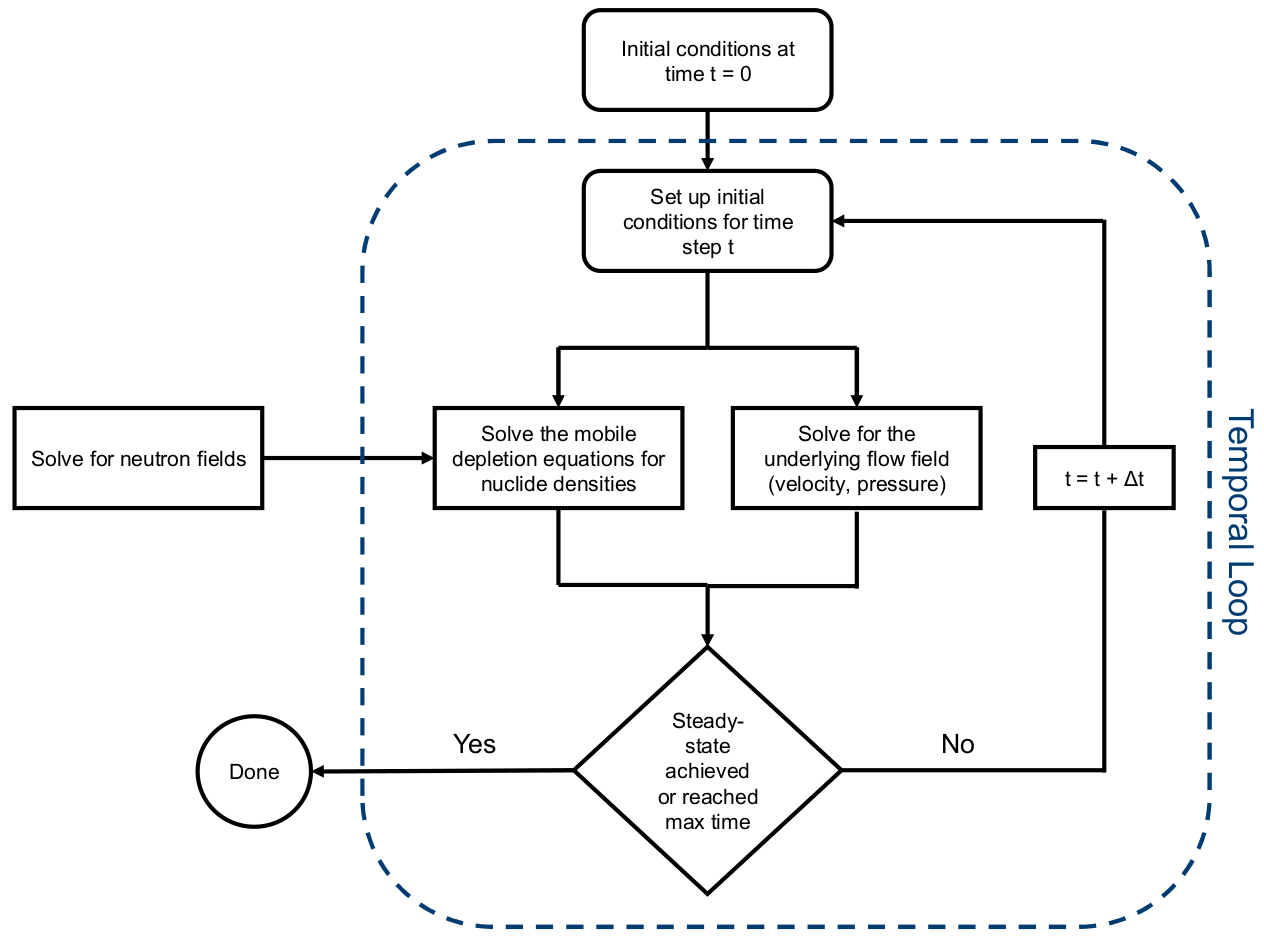
\includegraphics[width=0.95\textwidth]{images/solver/one_way.png}
    \caption{One-way solver coupling between neutron transport and mobile depletion.}
    \label{fig:solver:1_way}
\end{figure}

When considering photon transport for radiological consequence assessment and external dosimery, one must consider the rapid variation of the photon sources caused by the mobile depletion solver. This necessitates the inclusion of the photon transport solve within the inner temporal loop in Figure~\ref{fig:solver:1_way}, resulting in the following modified coupling scheme (Figure~\ref{fig:solver:1_way_photon_neutron}). The flexibility of the multi-app system within \acrshort{moose} allows for the exploration of several other coupling schemes, such as the use of sub-stepping for time integrating different physics over different time scales. This may prove to be useful with coupled photon transport and mobile depletion, as the mobile depletion equations can be sub-stepped with a shorter $\Delta t$ while the photon transport solve can utilize a longer timestep without encountering convergence issues.

\begin{figure}[H]
    \centering
    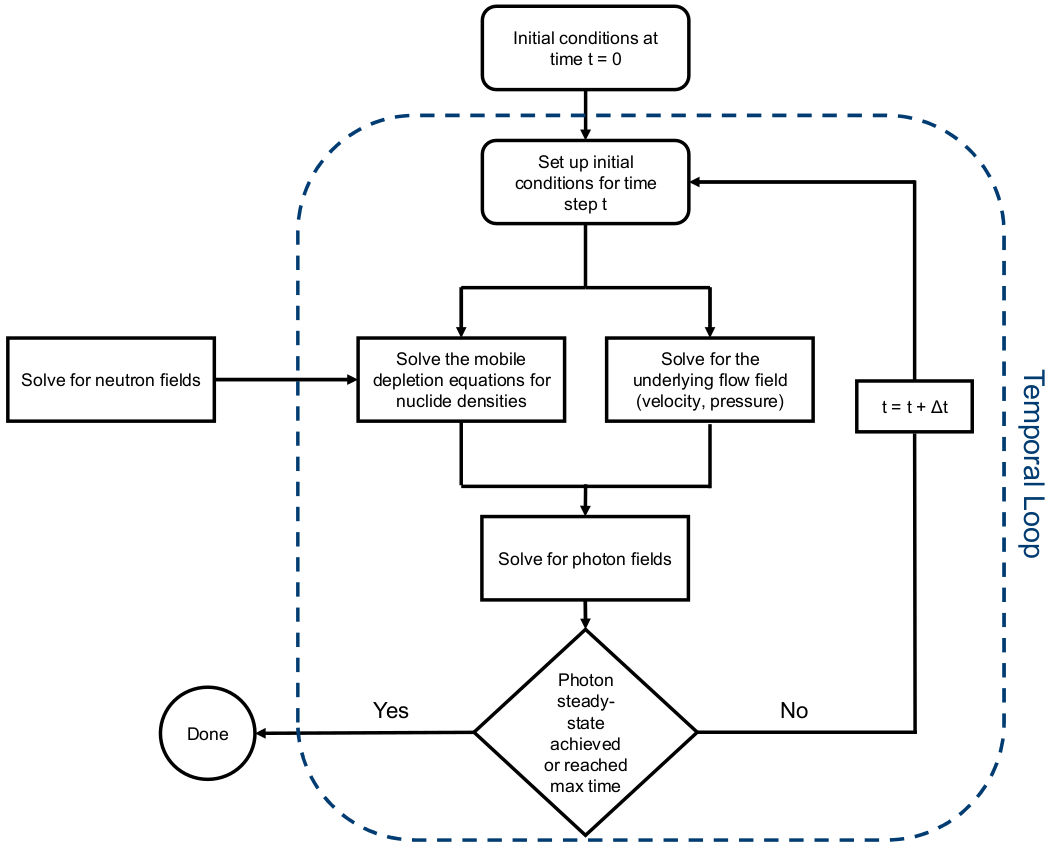
\includegraphics[width=0.95\textwidth]{images/solver/one_way_with_photon.png}
    \caption{Combined photon, neutron, and mobile depletion solver coupling strategy.}
    \label{fig:solver:1_way_photon_neutron}
\end{figure}

